% Options for packages loaded elsewhere
\PassOptionsToPackage{unicode}{hyperref}
\PassOptionsToPackage{hyphens}{url}
%
\documentclass[
  12pt,
]{article}
\usepackage{lmodern}
\usepackage{amssymb,amsmath}
\usepackage{ifxetex,ifluatex}
\ifnum 0\ifxetex 1\fi\ifluatex 1\fi=0 % if pdftex
  \usepackage[T1]{fontenc}
  \usepackage[utf8]{inputenc}
  \usepackage{textcomp} % provide euro and other symbols
\else % if luatex or xetex
  \usepackage{unicode-math}
  \defaultfontfeatures{Scale=MatchLowercase}
  \defaultfontfeatures[\rmfamily]{Ligatures=TeX,Scale=1}
  \setmainfont[]{Arial}
\fi
% Use upquote if available, for straight quotes in verbatim environments
\IfFileExists{upquote.sty}{\usepackage{upquote}}{}
\IfFileExists{microtype.sty}{% use microtype if available
  \usepackage[]{microtype}
  \UseMicrotypeSet[protrusion]{basicmath} % disable protrusion for tt fonts
}{}
\makeatletter
\@ifundefined{KOMAClassName}{% if non-KOMA class
  \IfFileExists{parskip.sty}{%
    \usepackage{parskip}
  }{% else
    \setlength{\parindent}{0pt}
    \setlength{\parskip}{6pt plus 2pt minus 1pt}}
}{% if KOMA class
  \KOMAoptions{parskip=half}}
\makeatother
\usepackage{xcolor}
\IfFileExists{xurl.sty}{\usepackage{xurl}}{} % add URL line breaks if available
\IfFileExists{bookmark.sty}{\usepackage{bookmark}}{\usepackage{hyperref}}
\hypersetup{
  pdftitle={Broadband connection and election in Brazil: what is role of the internet?},
  pdfauthor={Thiago Mendes Rosa},
  hidelinks,
  pdfcreator={LaTeX via pandoc}}
\urlstyle{same} % disable monospaced font for URLs
\usepackage[margin=1in]{geometry}
\usepackage{graphicx,grffile}
\makeatletter
\def\maxwidth{\ifdim\Gin@nat@width>\linewidth\linewidth\else\Gin@nat@width\fi}
\def\maxheight{\ifdim\Gin@nat@height>\textheight\textheight\else\Gin@nat@height\fi}
\makeatother
% Scale images if necessary, so that they will not overflow the page
% margins by default, and it is still possible to overwrite the defaults
% using explicit options in \includegraphics[width, height, ...]{}
\setkeys{Gin}{width=\maxwidth,height=\maxheight,keepaspectratio}
% Set default figure placement to htbp
\makeatletter
\def\fps@figure{htbp}
\makeatother
\setlength{\emergencystretch}{3em} % prevent overfull lines
\providecommand{\tightlist}{%
  \setlength{\itemsep}{0pt}\setlength{\parskip}{0pt}}
\setcounter{secnumdepth}{5}
\setlength\parindent{24pt}
\usepackage{indentfirst}
\usepackage{datetime}
\usepackage{setspace}
\onehalfspace
\usepackage{pdfpages}
\usepackage{floatrow}
\usepackage{amsmath}
\usepackage{bbm}
\usepackage{morefloats}
\usepackage{pbox}
\usepackage{graphicx}
\usepackage{tikz}
\usepackage{booktabs}
\usepackage{xcolor}
\usepackage{tabularx}
\floatplacement{figure}{H}
\floatsetup[figure]{capposition=top}
\floatsetup[table]{capposition=top}
\usepackage[bf]{caption}
\captionsetup{justification=raggedright,singlelinecheck=false}
\usepackage{placeins}
\usepackage{rotating}
\usepackage[hyphenbreaks]{breakurl}
\usepackage{pdflscape}
\usepackage{sectsty} \allsectionsfont{\centering}
\usepackage{tabu}
\usepackage{threeparttable}
\usepackage[normalem]{ulem}
\usepackage{makecell}
\usepackage{multirow}
\usepackage{afterpage}

\title{Broadband connection and election in Brazil: what is role of the
internet?}
\author{Thiago Mendes Rosa\footnote{Universidade de Brasília,
  \href{mailto:thiagomendesrosa@outlook.com}{\nolinkurl{thiagomendesrosa@outlook.com}}}}
\date{2020-09-02}

\begin{document}
\maketitle

\allsectionsfont{\centering}

\hypertarget{abstract}{%
\section*{Abstract}\label{abstract}}
\addcontentsline{toc}{section}{Abstract}

We investigate the relationship between broadband internet and election
outcomes in Brazil (2008, 2010 and 2012). Using a robust identification
strategy, a RDD applied to the roll out of Backhaul program, we explore
jumps in internet velocity according to population size as
identification strategy. Results indicate no relationship between
internet and political outcomes -- turnout, blank and null percentage
votes and left parties vote share. Our findings diverge from some
results reported before, usually applied to democracies with
institutional backgrounds distinct of the one observed in Brazil,
suggesting that this relationship may be context dependent.

\textbf{Keywords:} Internet, RDD, elections.

\allsectionsfont{\raggedright}

\clearpage

\hypertarget{introduction}{%
\section{Introduction}\label{introduction}}

The aim of this paper is to asses the impact of broadband connection
velocity on political outcomes: turnout, vote share, types of votes and
campaign donations.

The way how people get informed about politics has changed dramatically
over the years (Bimber 2003). If in XIX century press was the main
source of information, in the beginning of XX's radio took its place,
surpassed by television in the middle of the same century. Today, a new
type of media seems to be taking the lead: the internet .

Although the world wide web is an almost 30 years-old technology,
broadband connection is an even recent event (Maddux \& Johnson 1997).
Internet velocity capable of streaming videos became popular just in the
XXI century. Social networks, like Facebook, YouTube and Twitter are
relatively infant phenomenons\footnote{Facebook was launched in 2004,
  YouTube in 2005 and Twitter in 2006.}, becoming popular globally only
in the late of 2000's. Mobile broadband connections, thanks to 3G
technology (followed by 4G) and massification of smartphones, helped
internet to reach a greater number of users. New social medias, like
WhatsApp, Instagram and Telegram are now everyday tools\footnote{WhatsApp
  was launched in 2009, Instagram in 2010 and Telegram in 2013.}, with
popularity increasing in an exponential fashion, being common even for
business. A new wave, with 5G technology and the ``internet of things''
is coming to continue the revolution begun in the past century, with
connections speed and quality increasing every day, with new
possibilities of business.

Thus, information dissemination gained range and speed, reaching more
people, almost instantaneously, nearly in any part of the world.
Geographic barriers were broken and the amount of information are vast.
Before these new possibilities, a question arises: how this new scenario
affects social interaction? Furthermore, how do people are doing
politics in this new environment? In particular, if people have tools to
be more informed, do they increase their participation in elections?
Could vote preferences change with introduction of this new technology?
Or, on contrary, have this new possibilities of entertainment deviate
people from political discussion? Is it possible that internet did not
change politics at all?

These questions are not easy to be answered for several reasons.
Availability of internet is not random and characteristics like income,
schooling and geographic conditions may determine if an internet service
provider will be accessible for individuals (Falck \emph{et al.} 2014;
Miner 2015; Campante \emph{et al.} 2017). Also, institutional and
political backgrounds may possible influence internet-political
relationship.

This is not a novel issue. Relationship between internet and politics
has been focus of study in several fields(Bimber 1998; Larson 2004;
Czernich 2012; Jaber 2013; Falck \emph{et al.} 2014; Gavazza \emph{et
al.} 2015; Poy \& Schüller 2016; Campante \emph{et al.} 2017), and this
paper aims to contribute with this literature, studying internet impacts
on politics in Brazil. Focusing on a single country, we have best tools
to control possible confounders, and taking advantage of a specific rule
for broadband roll out, where number of inhabitants determines the
internet velocity of municipalities (the backhaul program), we have a
robust identification strategy, that creates an ideal instrument to deal
with internet velocity endogeneity. Following Cattaneo \emph{et al.}
(2018), we use multiple cutoffs design to estimate effects.

In the most recent Brazilian presidential election, internet had a major
role in result. In 2018, Mr.~Bolsonaro, with a little fraction of
financial resources used by his opponents\footnote{While Mr.~Bolsonaro
  expended R\$ 2.46 million in his campaign, the second place,
  Mr.~Haddad, expended R\% 37.5 million, a figure 15 times higher.
  Complete figures are available in
  \url{http://divulgacandcontas.tse.jus.br/}.} and with only eight
seconds of national advertising time in television\footnote{\url{https://agenciabrasil.ebc.com.br/politica/noticia/2018-08/tse-apresenta-tempos-de-radio-e-tv-de-presidenciaveis}}
he managed to go to the second round of presidential elections, with
46.03\% of votes, and won elections with a 10 p.p. difference. According
to Brazilian newspapers, the strength of Mr.~Bolsonaro in the social
medias was capital to his victory\footnote{\url{https://www.correiobraziliense.com.br/app/noticia/politica/2018/10/28/interna_politica,715584/bolsonaro-fez-das-redes-sociais-o-caminho-certo-para-uma-provavel-vito.shtml},
  \url{https://g1.globo.com/politica/blog/cristiana-lobo/post/2018/12/31/redes-sociais-mudam-completamente-a-relacao-dos-eleitores-com-seus-representantes.ghtml},
  \url{https://noticias.uol.com.br/politica/eleicoes/2018/noticias/2018/10/09/como-midias-sociais-e-orcamentos-enxutos-derrubaram-cinco-mitos-eleitorais.htm}},
which makes Brazil an interesting case of study regarding the
relationship between internet and elections.

Results suggests that, in general, broadband internet is not related to
political outcome in Brazil. It seems that internet did not influence
turnout, blank or null percentage votes and left parties vote share, in
2008, 2010 and 2012 elections, which covers national and local
elections. The office considered (president, mayor or deputies) did not
make difference in results. These finds are different from previous
results reported in the literature, meaning that institutional
background may play an important role in studies relating politics and
internet. Positive and negative relationship are reported for Germany,
Italy and United Kingdom (Falck \emph{et al.} 2014; Gavazza \emph{et
al.} 2015; Campante \emph{et al.} 2017), all of them with distinct
political institutional background compared with Brazilian's.

This paper is organized as follows: the first section presents the
theoretical framework linking internet to political outcomes, while the
next one reports the previous findings regarding its application. The
third section reviews the Brazilian political background, followed by
the section with empirical strategy, data bases and descriptive. The
fifth section presents our results, with a final discussion in the sixth
and last section.

\hypertarget{theoretical-framework}{%
\section{Theoretical framework}\label{theoretical-framework}}

There are some theories looking to explain why people vote (Downs 1957;
Riker \& Ordeshook 1968; Ferejohn \& Fiorina 1974; Uhlaner 1989; Aldrich
1993). One approach is to treat as a microeconomic problem in the
following way. In elections, individuals' problem is to choose the best
candidate(s) according to their preferences. But, there is an asymmetry
of information: there are many candidates (not considering uncontested
elections), and voters are not fully informed about their abilities.
Acquire information about them is costly, since they have to spend
resources to consume information (e.g.~from television, radio,
newspaper, internet or another people), that may include money and time.
Show up to cast the vote in the ballot also requires resources
(transportation and time, for example). More accurate decision requires
more information, which demands more resources, i.e.~is more costly. So,
it can be viewed as a maximization problem from the microeconomics point
of view, which can be solved by equalizing marginal costs and benefits.
Benefits can be viewed as the policies the most preferred candidate will
conduct, a civil duty or being party of the democratic process (Ali \&
Lin 2013).

This problem changes over time with entrance of new technologies
(Gentzkow 2006). For example, when radio, television and internet were
not available, there were fewer options to people get informed about
candidates. Also, there were available less leisure alternatives. With
emergence of radio, then television and, finally, internet, these costs
and substitution effects may have changed. A first natural question that
someone could have is: did these new technologies affect the decision of
voters? For newspaper, Gerber \emph{et al.} (2009), Gentzkow \emph{et
al.} (2011) and Drago \emph{et al.} (2014) report effects on elections
participation. According to Strömberg (2004) and Horacio \& Monteiro
(2014), radio affects people perception about politics, while DellaVigna
\& Kaplan (2007), Enikolopov \emph{et al.} (2011), Durante \& Knight
(2012), Gentzkow (2006) and Oberholzer-Gee \& Waldfogel (2009) shows the
impact of television (through news) on elections results.

How about the internet? Relationship between internet and politics has
been investigated since the end of 1990's (Bimber 1998). The effect on
information acquisition may be ambiguous depending on the hypothesis
used: if internet makes available new possibilities of entertainment,
people may substitute the time spent learning about politics with these
new type of leisure; on the other hand, if internet bring to people new
sources of politics information and channels of discussion, people may
be pushed toward politics. Finally, the cost and the time needed to find
candidates information or to find new possibilities of entertainment may
have changed relative prices. Once someone has access to internet, it is
possible to consume a variety of information with, in general, no
additional cost. The same is valid to leisure. A last possibility is
that the only thing substituted is the technology used to consume
information and leisure, making no difference in resources allocation at
all\footnote{If there is no, or little, consumption of politics
  information with an older technology, it might be the case that, even
  with a new technology, there is no preference for this type of
  information, resulting in no, or limited, shifting in its demand.}.

These changes may also take time to happen. Many types of media on
internet depends on broadband connection (like video streaming), only
available to the large public in the beginning of the XXI century.
Moreover, all content we have today were not available with the launch
of the internet. The same was true for television, where the diversity
of programs and shows existing today took time to be developed and
aired. Emergency of new technologies and its spread also affects
relative prices both for information and leisure over time with this
development.

While newspaper, radio and TV content production are more restricted and
with barrier entries, internet have opened doors to virtually anyone
produce information and media, interact with people and organize groups
of common interest, everything at a lower cost. Thus, it is likely to
exist a shift both in the demand and supply of information and
entertainment with internet arrival. It can potentially alter the manner
of how politics are made, since, with internet, politicians can reach
more people, quickly and at lower costs when compared with other medias.

One situation this new scenario brings is the social media consumption
of ``fake news''\footnote{Fake news is a term the popular term to
  define, in general, the spread of misleading or false information like
  if it were real. See Lazer \emph{et al.} (2018) for a brief
  discussion.} and its possible impact on elections. In the problem
treated here, misleading information may have a market that deviate
people from optimal choice (see Allcott \& Gentzkow 2017 for a
theoretical framework). Media capture by politicians put an additional
flavor to this discussion (Besley \& Prat 2006), where internet could
break other types of media control or enhance an existing control.

With this framework in mind, we analyze previous researches in the field
in order to collect results and identification strategies, pointing
resemblances and contrasts between them. Common outcomes between
internet and politics relationship are voting turnout, election results,
public polices and politician's accountability.

\hypertarget{literature}{%
\section{Literature}\label{literature}}

Sources from where people consume information and leisure are not
exogenous. For example, if television or internet is expensive, only
people with enough income can have access. If this kind of people have
particular preferences regarding candidates, then there is a bias if
relationship between internet and politic outcomes is treated as
unconditional. The same is valid for another characteristics, like race,
schooling, age or housing location.

Due to this endogeneity of internet supply and demand, geographical
characteristics (e.g landscape or rainfall) or previous
telecommunication infrastructure are common strategies taken to
instrumentalize internet in order to link it to political outcomes.
Campante \emph{et al.} (2017) study the impact broadband diffusion on
political participation for municipalities of Italy between 1996 and
2013 with this strategy. Miner (2015) take similar path for Malaysia,
Czernich (2012) and Falck \emph{et al.} (2014) for Germany, Gavazza
\emph{et al.} (2015) for UK, Jaber (2013) for USA and Menezes (2015) for
Brazil. With slightly different approach, Lelkes \emph{et al.} (2017)
explore variation in state laws related to internet infrastructure to
study influence of this technology on polarization in USA, while Poy \&
Schüller (2016) use similar strategy to analyse broadband effects on
turnout and vote share in rural and sparse areas in Italy.

For Italy, Campante \emph{et al.} (2017) report a negative effect on
turnout in elections following high speed internet implantation (2008),
changing its direction for later elections (2013). An interesting result
reported in Italian case is that internet affected ideological groups
distinctly, according to vote share results, paving the way for
organization of new political groups, formed in online platforms. Poy \&
Schüller (2016) echoes these results, linking high speed internet
(ADSL2+) to increases in turnout in 2008 and 2013 Italian elections, as
well transitory increases in vote share of some parties (center-left and
right-fringe).

In Malaysian case, Miner (2015) reports important effects of internet in
2008 election results (vote share of opposition parties), but not in
turnout and limited effects in turnover. It is interesting to note that
the political background for the Malaysian case is different from the
Italian one, although the identification strategy is similar.

A negative effect of internet on turnout is reported by Falck \emph{et
al.} (2014) for Germany. The mechanism is related to an increase in
leisure consumption that crowds out television entertainment, since
internet can be viewed as a substitute in this kind of
consumption\footnote{If we consider that people have a fixed amount of
  time to enjoy leisure activities, internet enters as a new option to
  compete with television, potentially reducing the time spent with the
  latter.}. The impact reported is heterogeneous: west Germany was
affect, while in east Germany no effect was observed, while effects on
vote shares were not observed in neither places. On the other hand,
Czernich (2012) found positive effects on participation in German
2002-2005 election.

Gavazza \emph{et al.} (2015) report for UK negative effects of internet
on turnout in 2006-2010 elections, with stronger results for
less-educated and younger voters. Furthermore, incumbents seems to take
advantage, diminishing election competitiveness. Taking a step further,
the UK study suggests effects on public policies, lowering public
expenses and taxes in areas with higher internet access (with similar
heterogeneity effects reported for turnout).

In Brazilian case, Menezes (2015) shows that internet is associated with
increases in vote share of small candidates in 2010 elections, but no
relation with turnout nor with no candidates votes (blank votes). This
is an important result once the winner of last Brazilian presidential
election (2018) won with a very limited advertisement time on radio and
television in the first round.

For USA, results presented by Lelkes \emph{et al.} (2017) seems to bring
light to mechanisms underlying the effects of internet one politics
outcomes. States with less restrictive laws (and more likely to have
broadband coverage) induces people to be exposed to partisan information
and be more extreme in partisan preferences. This mechanism is
compatible with results presented in Jaber (2013), who reports a
positive impact on turnout, donations to political campaigns and
democrats vote share in 2008 presidential elections. In an early study,
with weaker identification strategy, Tolbert \& McNeal (2003) suggests
that, in 1996 and 2000 presidential election, individuals with internet
and online elections news reading are more likely to vote.

It is important to note that countries have distinct political regimes,
which could potentially affect results reported. Minard \& Landriault
(2015) bring this to discussion analysing how maturity of democracy
regimes in Asia responds to internet availability. Immature regimes
seems to be more affect by internet than solid democracies according to
2006 cross-country analysis. Hence, the cross country variation suggests
that there are institutional factors playing action on internet-politics
relationship, which puts caution to external validity of results.

To sum up, it is clear that there are different results for different
countries (even inside the same country), with possible changing effects
over the time. Also, the majority of studies are concentrated in 2000
decade elections, focusing on the begging of the broadband internet. Few
studies report results for elections held in 2010 decade, when
smartphone revolution and social media gained strength. Even more, there
are no studies about the effects of mobile broadband and smartphones on
elections.

In this paper we will address fixed line broadband roll out, studying
the Brazilian case, one of the largest democracies in the world. As
pointed before, peculiarities of each country seems to be determinant
for results, which demands closer analysis of the political system in
order to compare our results with those presented before.

\hypertarget{brazilian-political-institutional-background}{%
\section{Brazilian political institutional
background}\label{brazilian-political-institutional-background}}

Brazil is a Federal Republic, with three layers of government: central
(or Federal), states and municipalities (see Souza (2005) for a
discussion about the federalism in Brazil). It is a young presidential
democracy, with bicameral legislative system (Chamber of Deputies and
Senate, the National Congress), holding election every four years.
President is elected by direct vote since 1989 in national elections, as
well national congress, state governors and state assemblies (1994
onward). Local elections, for municipal mayors and local legislators are
also held every four years, since 1996\footnote{Brazilian dictatorship
  ended in 1985, with general election in 1986, except for president
  (elected indirectly in the previous year). Before 1985, all other
  elections (except for president) had direct vote, but under military
  rules. In 1988, a new constitution was promulgated and in 1989 the
  president was elected by direct vote again, after 29 years. In 1990,
  there were elections for state governors, state assemblies and
  national congress. In 1992, municipal mayors and local assembly
  members were elected. By 1994 onward, national elections (president,
  state governors, state assembly and national congress) happens every
  four year, while local elections (municipal mayor and municipal
  assembly) happens every four years, since 1996. Thus, Brazil has
  elections every two years since 1994.}. While mayors, senators and the
president are elected in a majoritarian system, all the other candidates
are elected by proportional representation, where voters choose first a
party and then a candidate\footnote{There is the option to vote only for
  a party.}. Also, parties, until 2018, could create coalition\footnote{Altered
  by the Constitutional Amendment 45, available in
  \url{http://www.planalto.gov.br/ccivil_03/constituicao/Emendas/Emc/emc97.htm}}
to run in proportional elections, while in majoritarian elections,
coalitions are still permited. With this system, in 2018, 35 parties ran
in the elections. Table \ref{tab:parties} presents all parties and the
number of candidates that participated in elections from 2000 to 2018.

\begin{table}[H]

\caption{\label{tab:parties}Parties and number of candidates in Brazilian elections, 2000-2018}
\centering
\fontsize{9}{11}\selectfont
\begin{tabu} to \linewidth {>{\raggedright\arraybackslash}p{4cm}>{\raggedleft}X>{\raggedleft}X>{\raggedleft}X>{\raggedleft}X>{\raggedleft}X>{\raggedleft}X>{\raggedleft}X>{\raggedleft}X>{\raggedleft}X>{\raggedleft}X}
\toprule
Party & 2000 & 2002 & 2004 & 2006 & 2008 & 2010 & 2012 & 2014 & 2016 & 2018\\
\midrule
NOVO &  &  &  &  &  &  &  &  & 133 & 336\\
PAN & 414 & 287 & 597 & 359 &  &  &  &  &  & \\
PC do B & 261 & 73 & 478 & 215 & 633 & 581 & 1,251 & 589 & 674 & 585\\
PCB & 82 & 6 & 98 & 36 & 107 & 22 & 150 & 43 & 93 & 28\\
PCO & 28 & 71 & 156 & 41 & 16 & 3 & 6 & 12 & 15 & 11\\
PDT & 922 & 552 & 862 & 813 & 878 & 618 & 1,136 & 609 & 864 & 523\\
PEN/PATRIOTA &  &  &  &  &  &  &  & 625 & 893 & 862\\
PFL/DEM & 745 & 359 & 702 & 418 & 750 & 375 & 914 & 301 & 828 & 356\\
PGT & 417 & 368 &  &  &  &  &  &  &  & \\
PMB &  &  &  &  &  &  &  &  & 664 & 327\\
PMDB/MDB & 972 & 568 & 844 & 696 & 679 & 617 & 906 & 658 & 838 & 581\\
PMN & 516 & 154 & 657 & 359 & 532 & 403 & 785 & 312 & 850 & 462\\
PPB/PP & 805 & 423 & 806 & 346 & 693 & 445 & 1,013 & 363 & 790 & 439\\
PPL &  &  &  &  &  &  & 311 & 256 & 612 & 400\\
PPS/CIDADANIA & 841 & 514 & 810 & 665 & 893 & 490 & 1,151 & 382 & 909 & 369\\
PR/PL & 866 & 665 & 908 & 503 & 703 & 413 & 920 & 492 & 715 & 472\\
PRB/REPUBLICANOS &  &  &  & 54 & 534 & 363 & 858 & 436 & 928 & 608\\
PRN/PTC & 303 & 98 & 532 & 299 & 489 & 577 & 939 & 460 & 954 & 495\\
PRONA & 443 & 311 & 592 & 355 &  &  &  &  &  & \\
PROS &  &  &  &  &  &  &  & 215 & 659 & 831\\
PRP & 489 & 216 & 517 & 385 & 575 & 349 & 924 & 609 & 1,008 & 683\\
PRTB & 469 & 271 & 414 & 258 & 359 & 301 & 727 & 397 & 953 & 695\\
PSB & 878 & 739 & 960 & 703 & 756 & 697 & 1,135 & 789 & 827 & 488\\
PSC & 882 & 378 & 672 & 533 & 811 & 585 & 1,095 & 639 & 1,002 & 587\\
PSD & 511 & 244 &  &  &  &  & 679 & 303 & 907 & 362\\
PSDB & 717 & 427 & 815 & 534 & 838 & 520 & 934 & 606 & 981 & 439\\
PSDC/DC & 516 & 196 & 636 & 320 & 516 & 236 & 970 & 473 & 924 & 398\\
PSL & 480 & 222 & 611 & 284 & 666 & 559 & 868 & 472 & 934 & 935\\
PSN/PHS & 470 & 254 & 656 & 328 & 619 & 341 & 907 & 606 & 1,086 & 658\\
PSOL &  &  &  & 249 & 503 & 587 & 892 & 676 & 689 & 829\\
PST & 503 & 277 &  &  &  &  &  &  &  & \\
PSTU & 120 & 107 & 168 & 38 & 76 & 29 & 60 & 120 & 69 & 51\\
PT & 743 & 866 & 989 & 743 & 876 & 747 & 1,192 & 780 & 600 & 668\\
PT do B/AVANTE & 528 & 299 & 495 & 382 & 549 & 382 & 838 & 524 & 708 & 785\\
PTB & 963 & 526 & 722 & 581 & 804 & 609 & 942 & 583 & 908 & 389\\
PTN/PODEMOS & 396 & 129 & 625 & 215 & 611 & 373 & 1,037 & 377 & 1,125 & 598\\
PV & 656 & 478 & 1,017 & 752 & 875 & 918 & 1,194 & 726 & 1,029 & 581\\
REDE &  &  &  &  &  &  &  &  & 525 & 429\\
SD/SOLIDARIEDADE &  &  &  &  &  &  &  & 342 & 880 & 571\\
Total candidates & 16,936 & 10,078 & 17,339 & 11,464 & 16,341 & 12,140 & 24,734 & 14,775 & 26,574 & 17,831\\
Total parties & 30 & 30 & 27 & 29 & 27 & 27 & 29 & 32 & 35 & 35\\
\bottomrule
\multicolumn{11}{l}{\rule{0pt}{1em}Source: TSE}\\
\multicolumn{11}{l}{\rule{0pt}{1em}Obs.: Parties which changed their names are considered as an unique party.}\\
\end{tabu}
\end{table}

Considering that there are a large number of parties in Brazil, to make
the vote share analysis manageable, parties were classified as left,
center or right orientation based on Power \& Zucco Jr (2012) party
index\footnote{The authors construct a party index based on legislative
  surveys from 1990 to 2009, taking into consideration the ideological
  position of congress members in their activities.}. Table
\ref{tab:parties_orient} presents this organization.

\begin{table}[H]

\caption{\label{tab:parties_orient}Party classification according to orientation (left, center or right)}
\centering
\resizebox{\linewidth}{!}{
\begin{tabu} to \linewidth {>{\raggedright}X>{\raggedright}X>{\raggedright}X}
\toprule
Left & Center & Right\\
\midrule
PC do B & PCB & PFL/DEM\\
PCO & PDT & PMN\\
PSB & PMDB/MDB & PPB/PP\\
PSOL & PPL & PRN/PTC\\
PSTU & PPS/CIDADANIA & PRTB\\
PT & PR/PL & PSDC/DC\\
 & PRB/REPUBLICANOS & PSL\\
 & PRONA & \\
 & PRP & \\
 & PSC & \\
 & PSD & \\
 & PSDB & \\
 & PSN/PHS & \\
 & PT do B/AVANTE & \\
 & PTB & \\
 & PTN/PODEMOS & \\
 & PV & \\
 & SD/SOLIDARIEDADE & \\
\bottomrule
\multicolumn{3}{l}{\rule{0pt}{1em}Obs.: Division of parties based on quantiles of party index (0.25, 0.75, 1)}\\
\multicolumn{3}{l}{\rule{0pt}{1em}Obs.2: Parties out of party index were allocated based on party description available on their internet page.}\\
\end{tabu}}
\end{table}

The party index has some aggregation of parties as ``others'', so
another classification criterion was necessary. Parties web pages were
consulted to analyze their history and beliefs in order to designate
parties to the groups. This methodology may arise questions if some
parties labeled as right are actually centrists. To avoid this issue, we
focus on left parties vote shares in results section, since their
classification are more direct and mostly based on the party index.

The relatively large number of parties in Brazilian makes both elections
and politics complex processes (Pettersson-Lidbom 2008; Boulding \&
Brown 2015). In order to help understanding this process, Table
\ref{tab:ganhadores1} show the winners, by party, in the last five
elections, while Table \ref{tab:ganhadores2} shows the same information
for state governors and municipalities\footnote{Since 1988, Brazil has
  26 states and the Federal District. In 2018, there were 5,568
  municipalities, with two districts, the Federal capital and the state
  Fernando de Noronha, in Pernambuco. National Congress has 513 Federal
  Deputies and 81 Senators}.

\begin{table}[H]

\caption{\label{tab:ganhadores1}Distribuition of winners by party in National Congress, 2002-2018}
\centering
\resizebox{\linewidth}{!}{
\fontsize{9}{11}\selectfont
\begin{tabu} to \linewidth {>{\raggedright\arraybackslash}p{4cm}>{\raggedleft}X>{\raggedleft}X>{\raggedleft}X>{\raggedleft}X>{\raggedleft}X>{\raggedleft}X>{\raggedleft}X>{\raggedleft}X>{\raggedleft}X>{\raggedleft}X}
\toprule
\multicolumn{1}{c}{} & \multicolumn{2}{c}{2002} & \multicolumn{2}{c}{2006} & \multicolumn{2}{c}{2010} & \multicolumn{2}{c}{2014} & \multicolumn{2}{c}{2018} \\
\cmidrule(l{3pt}r{3pt}){2-3} \cmidrule(l{3pt}r{3pt}){4-5} \cmidrule(l{3pt}r{3pt}){6-7} \cmidrule(l{3pt}r{3pt}){8-9} \cmidrule(l{3pt}r{3pt}){10-11}
Party & Deputy & Senator & Deputy & Senator & Deputy & Senator & Deputy & Senator & Deputy & Senator\\
\midrule
NOVO & 0.0 & 0.0 & 0.0 & 0.0 & 0.0 & 0.0 & 0.0 & 0.0 & 1.6 & 0.0\\
PAN & 0.0 & 0.0 & 0.2 & 0.0 & 0.0 & 0.0 & 0.0 & 0.0 & 0.0 & 0.0\\
PC do B & 2.3 & 0.0 & 2.5 & 3.7 & 2.9 & 1.9 & 2.0 & 0.0 & 1.8 & 0.0\\
PDT & 4.1 & 7.4 & 4.7 & 3.7 & 5.3 & 3.7 & 3.9 & 14.8 & 5.5 & 3.7\\
PEN/PATRIOTA & 0.0 & 0.0 & 0.0 & 0.0 & 0.0 & 0.0 & 0.4 & 0.0 & 1.0 & 0.0\\
PFL/DEM & 16.4 & 25.9 & 12.7 & 22.2 & 8.4 & 3.7 & 4.1 & 11.1 & 5.7 & 7.4\\
PMB & 0.0 & 0.0 & 0.0 & 0.0 & 0.0 & 0.0 & 0.0 & 0.0 & 0.0 & 0.0\\
PMDB/MDB & 14.8 & 16.7 & 17.4 & 14.8 & 15.2 & 25.9 & 12.7 & 18.5 & 6.6 & 13.0\\
PMN & 0.2 & 0.0 & 0.6 & 0.0 & 0.8 & 1.9 & 0.6 & 0.0 & 0.6 & 0.0\\
PPB/PP & 9.4 & 0.0 & 8.0 & 3.7 & 8.6 & 7.4 & 7.4 & 3.7 & 7.2 & 9.3\\
PPL & 0.0 & 0.0 & 0.0 & 0.0 & 0.0 & 0.0 & 0.0 & 0.0 & 0.2 & 0.0\\
PPS/CIDADANIA & 2.9 & 1.9 & 4.3 & 3.7 & 2.3 & 1.9 & 2.0 & 0.0 & 1.6 & 3.7\\
PR/PL & 5.1 & 3.7 & 4.5 & 3.7 & 8.0 & 7.4 & 6.6 & 3.7 & 6.4 & 1.9\\
PRB/REPUBLICANOS & 0.0 & 0.0 & 0.2 & 0.0 & 1.6 & 1.9 & 4.1 & 0.0 & 5.8 & 1.9\\
PRN/PTC & 0.0 & 0.0 & 0.6 & 0.0 & 0.2 & 0.0 & 0.4 & 0.0 & 0.4 & 0.0\\
PRONA & 1.2 & 0.0 & 0.4 & 0.0 & 0.0 & 0.0 & 0.0 & 0.0 & 0.0 & 0.0\\
PROS & 0.0 & 0.0 & 0.0 & 0.0 & 0.0 & 0.0 & 2.1 & 0.0 & 1.6 & 1.9\\
PRP & 0.0 & 0.0 & 0.0 & 0.0 & 0.4 & 0.0 & 0.6 & 0.0 & 0.8 & 1.9\\
PRTB & 0.0 & 0.0 & 0.0 & 3.7 & 0.4 & 0.0 & 0.2 & 0.0 & 0.0 & 0.0\\
PSB & 4.3 & 5.6 & 5.3 & 3.7 & 6.8 & 7.4 & 6.6 & 11.1 & 6.2 & 3.7\\
PSC & 0.2 & 0.0 & 1.8 & 0.0 & 3.3 & 1.9 & 2.5 & 0.0 & 1.6 & 1.9\\
PSD & 0.8 & 1.9 & 0.0 & 0.0 & 0.0 & 0.0 & 7.0 & 7.4 & 6.6 & 7.4\\
PSDB & 13.7 & 14.8 & 12.9 & 18.5 & 10.5 & 11.1 & 10.5 & 14.8 & 5.7 & 7.4\\
PSDC/DC & 0.2 & 0.0 & 0.0 & 0.0 & 0.0 & 0.0 & 0.4 & 0.0 & 0.2 & 0.0\\
PSL & 0.2 & 0.0 & 0.0 & 0.0 & 0.2 & 0.0 & 0.2 & 0.0 & 10.1 & 7.4\\
PSN/PHS & 0.0 & 0.0 & 0.4 & 0.0 & 0.4 & 0.0 & 1.0 & 0.0 & 1.2 & 3.7\\
PSOL & 0.0 & 0.0 & 0.6 & 0.0 & 0.6 & 1.9 & 1.0 & 0.0 & 2.0 & 0.0\\
PST & 0.6 & 0.0 & 0.0 & 0.0 & 0.0 & 0.0 & 0.0 & 0.0 & 0.0 & 0.0\\
PT & 17.7 & 18.5 & 16.2 & 7.4 & 16.8 & 20.4 & 13.4 & 7.4 & 10.9 & 7.4\\
PT do B/AVANTE & 0.0 & 0.0 & 0.2 & 0.0 & 0.6 & 0.0 & 0.2 & 0.0 & 1.4 & 0.0\\
PTB & 5.1 & 3.7 & 4.3 & 11.1 & 4.3 & 1.9 & 4.9 & 7.4 & 2.0 & 3.7\\
PTN/PODEMOS & 0.0 & 0.0 & 0.0 & 0.0 & 0.0 & 0.0 & 0.8 & 0.0 & 2.1 & 1.9\\
PV & 1.0 & 0.0 & 2.5 & 0.0 & 2.5 & 0.0 & 1.6 & 0.0 & 0.8 & 0.0\\
REDE & 0.0 & 0.0 & 0.0 & 0.0 & 0.0 & 0.0 & 0.0 & 0.0 & 0.2 & 9.3\\
SD/SOLIDARIEDADE & 0.0 & 0.0 & 0.0 & 0.0 & 0.0 & 0.0 & 2.9 & 0.0 & 2.5 & 1.9\\
\bottomrule
\multicolumn{11}{l}{\rule{0pt}{1em}Source: TSE}\\
\multicolumn{11}{l}{\rule{0pt}{1em}Obs.: Parties which changed their names are considered as an unique party.}\\
\end{tabu}}
\end{table}

\begin{table}[H]

\caption{\label{tab:ganhadores2}Distribuition of winners by party in National Congress, 2002-2018}
\centering
\resizebox{\linewidth}{!}{
\fontsize{9}{11}\selectfont
\begin{tabu} to \linewidth {>{\raggedright\arraybackslash}p{4cm}>{\raggedleft}X>{\raggedleft}X>{\raggedleft}X>{\raggedleft}X>{\raggedleft}X>{\raggedleft}X>{\raggedleft}X>{\raggedleft}X>{\raggedleft}X>{\raggedleft}X}
\toprule
\multicolumn{1}{c}{} & \multicolumn{2}{c}{2000/2002} & \multicolumn{2}{c}{2004/2006} & \multicolumn{2}{c}{2008/2010} & \multicolumn{2}{c}{2012/2014} & \multicolumn{2}{c}{2016/2018} \\
\cmidrule(l{3pt}r{3pt}){2-3} \cmidrule(l{3pt}r{3pt}){4-5} \cmidrule(l{3pt}r{3pt}){6-7} \cmidrule(l{3pt}r{3pt}){8-9} \cmidrule(l{3pt}r{3pt}){10-11}
Party & Mayor & Gov. & Mayor & Gov. & Mayor & Gov. & Mayor & Gov. & Mayor & Gov.\\
\midrule
NOVO & 0.0 & 0.0 & 0.0 & 0.0 & 0.0 & 0.0 & 0.0 & 0.0 & 0.0 & 3.7\\
PAN & 0.0 & 0.0 & 0.0 & 0.0 & 0.0 & 0.0 & 0.0 & 0.0 & 0.0 & 0.0\\
PC do B & 0.0 & 0.0 & 0.2 & 0.0 & 0.7 & 0.0 & 1.0 & 3.6 & 1.5 & 3.7\\
PDT & 5.4 & 3.7 & 5.5 & 7.4 & 6.3 & 0.0 & 5.5 & 7.1 & 6.0 & 3.7\\
PEN/PATRIOTA & 0.0 & 0.0 & 0.0 & 0.0 & 0.0 & 0.0 & 0.0 & 0.0 & 0.2 & 0.0\\
PFL/DEM & 18.6 & 14.8 & 14.2 & 3.7 & 8.9 & 7.4 & 5.0 & 0.0 & 4.9 & 7.4\\
PMB & 0.0 & 0.0 & 0.0 & 0.0 & 0.0 & 0.0 & 0.0 & 0.0 & 0.1 & 0.0\\
PMDB/MDB & 22.2 & 18.5 & 19.0 & 25.9 & 21.7 & 18.5 & 18.4 & 25.0 & 18.9 & 11.1\\
PMN & 0.3 & 0.0 & 0.6 & 0.0 & 0.8 & 3.7 & 0.7 & 0.0 & 0.5 & 0.0\\
PPB/PP & 11.0 & 0.0 & 9.9 & 3.7 & 9.9 & 0.0 & 8.6 & 3.6 & 9.0 & 3.7\\
PPL & 0.0 & 0.0 & 0.0 & 0.0 & 0.0 & 0.0 & 0.2 & 0.0 & 0.1 & 0.0\\
PPS/CIDADANIA & 3.0 & 7.4 & 5.5 & 7.4 & 2.3 & 0.0 & 2.2 & 0.0 & 2.2 & 0.0\\
PR/PL & 4.2 & 0.0 & 6.8 & 0.0 & 6.9 & 0.0 & 5.0 & 0.0 & 5.4 & 0.0\\
PRB/REPUBLICANOS & 0.0 & 0.0 & 0.0 & 0.0 & 1.0 & 0.0 & 1.4 & 0.0 & 1.9 & 0.0\\
PRN/PTC & 0.1 & 0.0 & 0.3 & 0.0 & 0.2 & 0.0 & 0.4 & 0.0 & 0.3 & 0.0\\
PRONA & 0.0 & 0.0 & 0.1 & 0.0 & 0.0 & 0.0 & 0.0 & 0.0 & 0.0 & 0.0\\
PROS & 0.0 & 0.0 & 0.0 & 0.0 & 0.0 & 0.0 & 0.0 & 3.6 & 0.9 & 0.0\\
PRP & 0.3 & 0.0 & 0.7 & 0.0 & 0.3 & 0.0 & 0.4 & 0.0 & 0.3 & 0.0\\
PRTB & 0.1 & 0.0 & 0.2 & 0.0 & 0.2 & 0.0 & 0.3 & 0.0 & 0.2 & 0.0\\
PSB & 2.6 & 14.8 & 3.1 & 11.1 & 5.6 & 22.2 & 7.9 & 10.7 & 7.4 & 11.1\\
PSC & 0.5 & 0.0 & 0.4 & 0.0 & 1.0 & 0.0 & 1.5 & 0.0 & 1.6 & 7.4\\
PSD & 1.9 & 0.0 & 0.0 & 0.0 & 0.0 & 0.0 & 8.9 & 7.1 & 9.7 & 7.4\\
PSDB & 17.6 & 25.9 & 15.7 & 22.2 & 14.3 & 29.6 & 12.5 & 21.4 & 14.5 & 11.1\\
PSDC/DC & 0.1 & 0.0 & 0.2 & 0.0 & 0.1 & 0.0 & 0.2 & 0.0 & 0.1 & 0.0\\
PSL & 0.5 & 3.7 & 0.4 & 0.0 & 0.3 & 0.0 & 0.4 & 0.0 & 0.5 & 11.1\\
PSN/PHS & 0.1 & 0.0 & 0.4 & 0.0 & 0.2 & 0.0 & 0.3 & 0.0 & 0.7 & 3.7\\
PSOL & 0.0 & 0.0 & 0.0 & 0.0 & 0.0 & 0.0 & 0.0 & 0.0 & 0.0 & 0.0\\
PST & 0.2 & 0.0 & 0.0 & 0.0 & 0.0 & 0.0 & 0.0 & 0.0 & 0.0 & 0.0\\
PT & 3.5 & 11.1 & 7.4 & 18.5 & 10.0 & 18.5 & 11.5 & 17.9 & 4.6 & 14.8\\
PT do B/AVANTE & 0.1 & 0.0 & 0.4 & 0.0 & 0.1 & 0.0 & 0.4 & 0.0 & 0.2 & 0.0\\
PTB & 7.5 & 0.0 & 7.6 & 0.0 & 7.4 & 0.0 & 5.3 & 0.0 & 4.6 & 0.0\\
PTN/PODEMOS & 0.0 & 0.0 & 0.1 & 0.0 & 0.3 & 0.0 & 0.2 & 0.0 & 0.5 & 0.0\\
PV & 0.2 & 0.0 & 1.0 & 0.0 & 1.4 & 0.0 & 1.8 & 0.0 & 1.8 & 0.0\\
REDE & 0.0 & 0.0 & 0.0 & 0.0 & 0.0 & 0.0 & 0.0 & 0.0 & 0.1 & 0.0\\
SD/SOLIDARIEDADE & 0.0 & 0.0 & 0.0 & 0.0 & 0.0 & 0.0 & 0.0 & 0.0 & 1.1 & 0.0\\
\bottomrule
\multicolumn{11}{l}{\rule{0pt}{1em}Source: TSE}\\
\multicolumn{11}{l}{\rule{0pt}{1em}Obs.: Parties which changed their names are considered as an unique party.}\\
\end{tabu}}
\end{table}

Table \ref{tab:ganhadores1} shows that no party had more than 20\% of
the deputies. The workers party (PT), who won four out of five last
elections (2002 to 2014), did not have the majority of the congress in
any year.In the Senate, the party with more seats had around 1/4 of the
house until 2010, with more competitive elections since then, specially
in 2018. So, in order to run the country, the president needs to build
alliance, otherwise it is unlikely to pass its bills. The number of
parties necessary to form at least 60\% of the deputies\footnote{Bills
  that alter constitution require at least 308 votes of deputies and 49
  votes of senators, i.e.~60\% of the National Congress, in two rounds.}
has risen from four to eight, including both situation and opposition
parties, which means that the necessary number of parties required to
rule is even higher. In the senate, the number has risen from three to
seven.

Competitiveness observed in National Congress elections is also present
in subnational suffrage. Table \ref{tab:ganhadores2} shows that most
dominant party has around 20\% of mayors and 25\% of governors, not
necessary the same party in each election, adding another layer of
complexity in the Brazilian Federal System (see Cancela \& Geys (2016)
for a discussion about coordination in multilevel elections in Brazil).

Until 2017, parties had the Party Fund\footnote{The \emph{Fundo
  Partidário}, created by the Law 9,096/1995, available in
  \url{http://www.tse.jus.br/legislacao/codigo-eleitoral/lei-dos-partidos-politicos/lei-dos-partidos-politicos-lei-nb0-9.096-de-19-de-setembro-de-1995}.}
and private donations (since 2016, companies are not allowed to donate
for elections\footnote{According to a Supreme Court (STF) decision, ADI
  4,650/2015 and the Law 13,165/2015. Available in
  \url{http://redir.stf.jus.br/paginadorpub/paginador.jsp?docTP=TP&docID=10329542}
  and
  \url{http://www.planalto.gov.br/ccivil_03/_Ato2015-2018/2015/Lei/L13165.htm}}),
which includes own resources from candidates. There are maximum values
allowed to be expend by candidates in campaign, stipulated each year by
the Supreme Electoral Court (TSE - \emph{Supreto Tribunal Eleitoral}).
The Party Fund is distributed by the following rule: 5\% is equally
given to registered parties\footnote{In 2017, the Constitution Amend 33
  created the rules to access the Party Fund, so called \emph{Cláusula
  de Barreira} (Barrier Clause). In 2019, the party must had 1.5\% of
  valid votes for deputies in 2018, distributed at least in 1/3 of the
  states and with at least 1\% of the votes in each one, or had nine
  deputies in at least 1/3 of the states. This rule will be more rigid
  in 2023, with 2\% of the votes or 11 deputies, under the same rules.
  In 2027, the figures will be 2.5\% (and at least 1.5\% in 1/3 of the
  states) or 13 deputies and in 2031, they will be 3\% (and at least 2\%
  in 1/3 of the state) or 15 deputies.} and 95\% according to votes won
in the last deputies elections. In 2017, with prohibition of companies
donation, another fund was created, the Electoral Fund\footnote{Called
  \emph{Fundo Especial de Financiamento de Campanha}, it was created by
  the Laws 13,487/2017 and 13,488/2017. Available in
  \url{http://www.planalto.gov.br/ccivil_03/_Ato2015-2018/2017/Lei/L13487.htm}
  and
  \url{http://www.planalto.gov.br/ccivil_03/_ato2015-2018/2017/lei/L13488.htm}.},
which is distributed with following rule: 2\% equally between registered
parties; 35\% to parties with, at least, one deputy; 48\% according to
deputies proportion; and 15\% according to senators proportion. For
example, in 2018, the Fund Party was R\$ 888.7 million (US\$ 165
million), while the Electoral Fund was R\$ 1.7 billion (US\$ 316.3
million).

Another important aspect of Brazilian suffrage regards campaign
advertisement. There are national, free of charges and mandatory
programs during campaign time, booth aired daily in radio and
television, broadcasting the same content in all regions of the country.
There is a fixed amount of time for electoral advertisement in these
channels, 2/3 distributed according to current party presence in
legislatures and 1/3 among candidates\footnote{The same rules of the
  \emph{Cláusula de Barreira} (Barrier Clause) is also applied here.},
and only this time is allowed to be used in these channels. Ads on
newspaper are also restricted, even though being a less important media
compared to TV and radio. Internet is exception, where candidates can
use it, almost freely, to reach voters, since 2009, except for
anonymously or paid advertisement (which includes social medias like
Twitter, Facebook, Instagram and YouTube)\footnote{There is a set of
  other rules stipulated by the Supreme Electoral Court in each
  election, like size of advertisement material, schedule for rallies
  etc.}.

So, all this set of rules concentrate resources for some parties and
candidates, making the internet an important alternative in elections.
As aforementioned, in the presidential election of 2018, internet was
pointed out as crucial for the result.

Looking now to electorate, in Brazil, voting is mandatory to literate
citizens aged 18 to 69. For people aged 16 to 17 and 70 and over, voting
is optional. Voters absent in election must justify or pay a small fine.
If they fail to justify three consecutive polls, voter registration is
canceled and some rights are lost (issue or renew passports and national
identification, receive wages as public servant or from any institution
linked to government, participate in public competition for resources,
request loans from institutions held by the government, apply to jobs as
public servant, enroll in public education or engage in any public act
that requests military service or income task discharge). This set
raises the question if this rule changes incentives to acquire
information about politicians and participate in elections. Table
\ref{tab:cancelados} shows the total number of voters as well total
population with voter registration canceled from 2005 to 2019.

\begin{table}[H]

\caption{\label{tab:cancelados}Total of volters and voter registration canceled, 2005 to 2009}
\centering
\fontsize{9}{11}\selectfont
\begin{tabu} to \linewidth {>{\raggedright\arraybackslash}p{4cm}>{\raggedleft}X>{\raggedleft}X>{\raggedleft}X>{\raggedleft}X>{\raggedleft}X}
\toprule
Year & Voters & Turnout & Turnout \% & Canceled & Canceled \%\\
\midrule
2005 & 121,391,631 & 102,526,992 & 84.46 & 1,089,662 & 0.89\\
2007 & 125,913,494 & 104,820,459 & 83.25 & 1,652,565 & 1.30\\
2009 & 130,604,430 & 110,085,172 & 84.29 & 553,406 & 0.42\\
2011 & 135,804,433 & 111,193,747 & 81.88 & 1,400,549 & 1.03\\
2013 & 140,646,483 & 115,807,514 & 82.34 & 1,358,901 & 0.96\\
2015 & 142,822,083 & 115,122,883 & 80.61 & 1,717,425 & 1.20\\
2017 & 146,470,911 & 118,757,780 & 81.08 & 1,862,665 & 1.27\\
2019 & 147,306,275 & 117,364,654 & 79.67 & 2,491,271 & 1.69\\
\bottomrule
\multicolumn{6}{l}{\rule{0pt}{1em}Source: TSE}\\
\multicolumn{6}{l}{\rule{0pt}{1em}Obs.1: Includes voters registered in Brazil and abroad.}\\
\multicolumn{6}{l}{\rule{0pt}{1em}Obs.2: Turnout in the last elections.}\\
\end{tabu}
\end{table}

Despite the mandatory voting rule, turnout was 82.2\% in average from
2004 to 2018, and only 1.09\% of voters registration were canceled,
which means that more than 90\% of those who did not turnout took
actions to regularize their electoral obligations. Anyhow, turnout is
pretty high when compared to USA or European countries.

According to Downs (1957), low probability to be pivotal in elections
explain the ``rational ignorance'' of voters and low preference to turn
out. On the other hand, mandatory vote could change these incentives,
making people more inclined to vote (Lijphart 1997). Leon \emph{et al.}
(2014) finds that, for Brazilian case, mandatory voting seems not change
people incentives to be more informed in voting decision. It seems the
case that providing more information about candidates (Banerjee \emph{et
al.} 2011), hence lowering the costs for collect information, is more
effective than compulsory voting system.

Following Fujiwara \emph{et al.} (2016), we also consider possible
persistent habits on voting pattern, incorporating raining information
in election days in each municipality. The authors find that rainfall,
both in current and past election day, reduces turnout and may possible
affect consumption value of voting. Considering the continental size of
Brazil, it may be an important contribution for analysis.

\hypertarget{empirical-strategy-and-databases}{%
\section{Empirical strategy and
databases}\label{empirical-strategy-and-databases}}

In this section we describe in detail the empirical strategy, relied on
the Backhaul program rules, and the databases that support the analysis.

\hypertarget{communication-usage}{%
\subsection{Communication usage}\label{communication-usage}}

As a glimpse of Brazilian communication consumption, Figure \ref{fig:0}
presents internet and cell phone usage from 2008 to 2017.

\begin{figure}
\centering
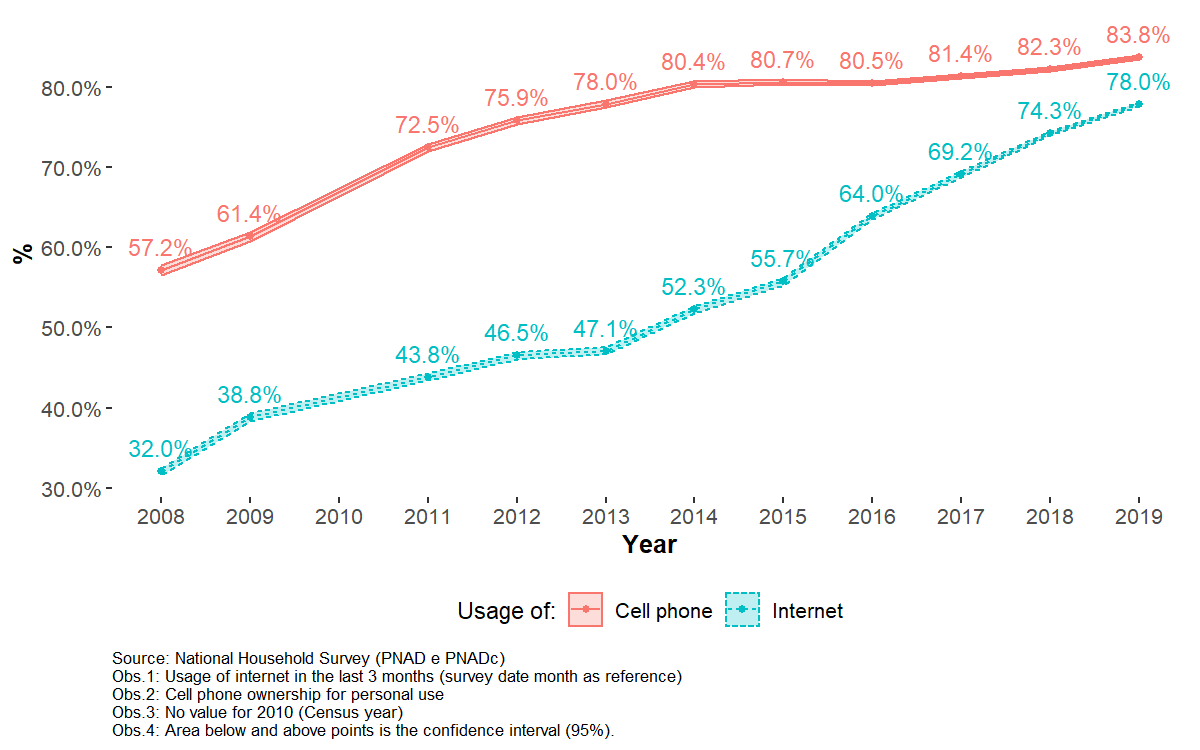
\includegraphics{artigo1_files/figure-latex/internet_usage-1.png}
\caption{Internet and cell phone usage in Brazil, \% of 16+ years-old
population, 2008-2009 and 2011-2017 \label{fig:0}}
\end{figure}

In 2008, around 1/3 of Brazilians (16 years-old or above,
i.e.~population in voting age) declared to have used internet at least
once in the last three months (September as reference), while almost
58\% declared cell phone ownership for personal usage. In order to
increase these figures, the government carried out a national plan in
the begging of 2008. In 2011, these figures rose to 44\% and 73\%,
respectively, indicating an increasing communication market in Brazil.
Even in 2018, there is room remaining for internet and cell phone
expansion in the country (around 25\% and 18\%, respectively).

Hence, this expressive change in communication consumption may have
changed how Brazilians face politics, possibly increasing opportunities
for information acquisition and social interaction about this matter,
or, on the other hand, widening leisure alternatives and lowering
politics information consumption.

\hypertarget{backhaul-program-national-broadband-plan}{%
\subsection{Backhaul Program (National Broadband
Plan)}\label{backhaul-program-national-broadband-plan}}

In April 2008, the presidential Decree 6,424 changed the former National
Plan of Goals for Public Switched Telephone (PST) Network
Universalization, adding broadband infrastructure as mandatory (in
exchange of the PST obligation). The infrastructure mentioned in the
Decree was the Backhaul, a requirement for internet implementation in
the country. Backhauls are necessary in order to connect them to the
Telephone Companies' Backbones. The plan put as target that, at least,
40\% of municipalities should have the necessary infrastructure by the
end of 2008, 80\% by the end of 2009 and 100\% by the end of 2010. Also,
minimal internet velocities were set, increasing with population size
(Table \ref{tab:program_backhauk}).

\begin{table}[H]

\caption{\label{tab:program_backhauk}Backhaul Plan --  setup}
\centering
\begin{tabu} to \linewidth {>{\raggedright\arraybackslash}p{5.cm}>{\raggedleft}X>{\raggedleft}X>{\raggedleft}X}
\toprule
Population Size & N\# municipalities & \% & Velocity (Mbps)\\
\midrule
Up to 20,000 & 3,077 & 90 & 8\\
From 20,001 to 40,000 & 268 & 8 & 16\\
From 40,001 to 60,000 & 63 & 2 & 32\\
Above 60,001 & 31 & 1 & 64\\
Total & 3,439 & 100 & \\
\bottomrule
\multicolumn{4}{l}{\rule{0pt}{1em}Source: Anatel}\\
\end{tabu}
\end{table}

According to the National Agency of Telecommunication (Anatel\footnote{\emph{Agência
  Nacional de Telecomunicações} in Portuguese.}) (Anatel 2010), the
majority of municipalities to be covered by Backhaul program were up to
20,0000 inhabitants, which is more than half of total municipalities of
Brazil\footnote{Today, Brazil has 5,570 municipalities. By the time when
  the program was created, six municipalities did not exist yet.}. The
minimal required velocity (8 Mbps\footnote{Megabit per second.})
guarantee improvement in navigation quality, allowing, for example,
streaming (music and videos).

The program had three types of technology to be deployed: fiber, radio
and satellite. The first is installed by cables of fiver optic, with
less interference and in higher distances, being connected directly to
the household (FTTH) or to a concentrating point (FTTC), either with a
higher cost of installation and maintenance. The second one is usually
easier to be installed, by antennas, maintained and reaches broader
areas, like rural locales, but have limitations of interference, due to
physical barriers, and in internet velocity, due to distance. Finally,
the third needs a satellite, an antenna in the household and a base
antenna to intermediate communication, a set with high costs of
installation and maintenance, but capable to reach broader areas, like
rural, and being susceptible to weather interference. Considering the
cost, radio was the main technology chosen, for 71\% of the cities,
followed by fiber, for 26\%, and satellite for only 3\%.

Out of 5,570 municipalities, by 2015, only 85 remained uncovered (Table
\ref{tab:desc_back}) and 2,125 (38\%) already had broadband
infrastructure before the program, mainly larger cities. We notice that
the program focused on small cities, with average population under
15,000.

\begin{table}[H]

\caption{\label{tab:desc_back}Backhaul deployment by coverage status, 2015}
\centering
\begin{tabu} to \linewidth {>{\raggedright}X>{\raggedleft}X>{\raggedleft}X}
\toprule
Situation & \# Munic & Avg Pop.\\
\midrule
Covered & 3,360 & 14,403\\
Covered before & 2,125 & 67,151\\
Uncovered & 85 & 35,372\\
Total & 5,570 & 34,072\\
\bottomrule
\multicolumn{3}{l}{\rule{0pt}{1em}Source: Anatel and IBGE}\\
\end{tabu}
\end{table}

According to program schedule, 100\% of Brazilians' municipalities
should has backhaul infrastructure in 2010. However, by this year, only
72\% of the goal was achieved. Table \ref{tab:backhaul_implementation}
presents the roll out of the program by year.

\begin{table}[H]

\caption{\label{tab:backhaul_implementation}Backhaul deployment by year}
\centering
\begin{tabu} to \linewidth {>{\raggedright}X>{\raggedleft}X>{\raggedleft}X>{\raggedleft}X}
\toprule
Backhaul year & \# Munic & Avg. Velocity & Avg Pop.\\
\midrule
2008 & 1,384 & 13 & 16,911\\
2009 & 1,388 & 10 & 13,340\\
2010 & 495 & 9 & 9,026\\
2011 & 27 & 2 & 12,134\\
2012 & 7 & 14 & 25,531\\
2013 & 41 & 4 & 20,238\\
2014 & 17 &  & 38,490\\
2015 & 1 &  & 13,293\\
Total & 3,360 & 11 & 14,403\\
\bottomrule
\multicolumn{4}{l}{\rule{0pt}{1em}Source: Anatel.}\\
\multicolumn{4}{l}{\rule{0pt}{1em}Obs.1: No velocity information for 2014 and 2015.}\\
\multicolumn{4}{l}{\rule{0pt}{1em}Obs.2: Information only for program participants cities.}\\
\end{tabu}
\end{table}

The main point of our identification strategy relies on the velocity
discontinuity, which is further analyzed in Figure \ref{fig:1}
geographically,\footnote{Since Brazil is a continental country with
  important regional inequalities, regional visualization improve
  analysis.}. North and Northeast regions are poorer, while South and
Southeast are richer\footnote{For example, the state of São Paulo was
  responsible for almost 1/3 of Brazilian GDP in 2017. Per capita
  household income of the richest state (Federal District) was 3.84
  times greater than the poorest (Alagoas), according to 2014 National
  Household Survey (IBGE/PNAD). Brazilian Gini index for the same year
  was 0.517.}, being important to analyze how the programs are deployed
in the territory.

\begin{figure}
\centering
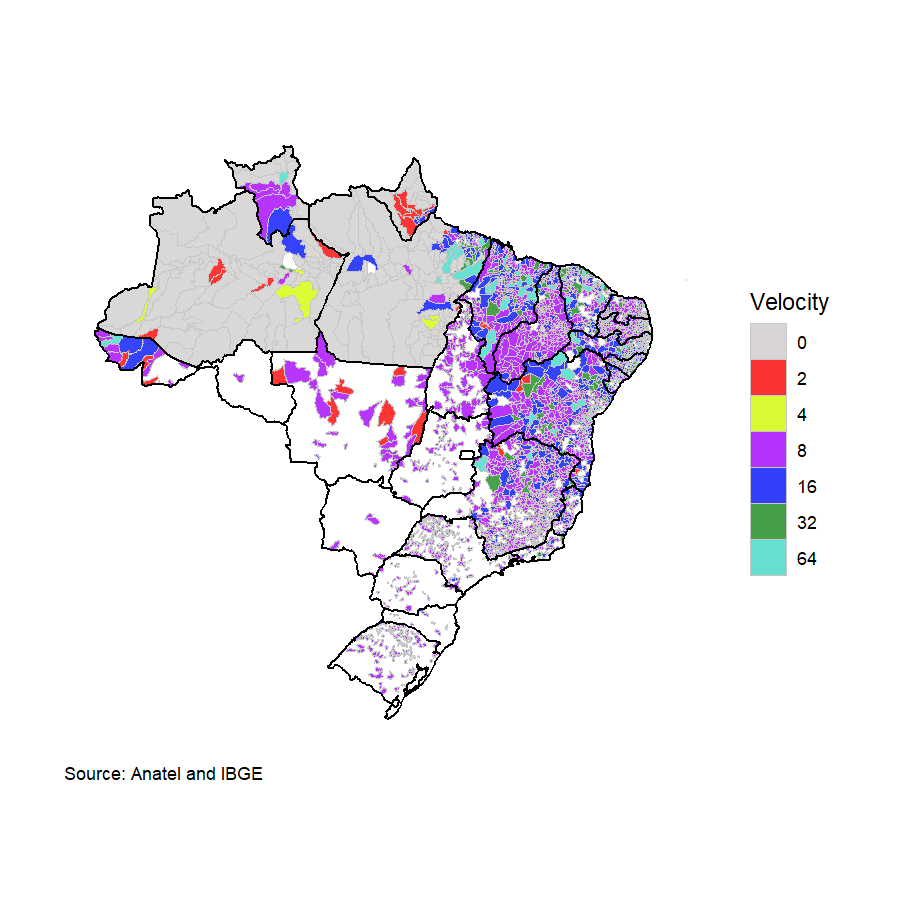
\includegraphics{artigo1_files/figure-latex/unnamed-chunk-2-1.png}
\caption{Internet velocity in backhaul program by municipality
\label{fig:1}}
\end{figure}

Figure \ref{fig:1} shows that a big portion of cities in the south and
center-west were covered before (blank areas), while the northeast had
the largest number of cities in the program. Also, the north region (the
Amazon area) had a lot of cities uncovered by the program (grey areas).
The most common velocity was 8 Mbps, as showed before in Table
\ref{tab:program_backhauk}, corresponding to cities under 20,000
inhabitants.

\hypertarget{methodology}{%
\subsection{Methodology}\label{methodology}}

Following Cattaneo \emph{et al.} (2018), each municipality has a running
variable \(X_i\) (the size of population) with potential outcomes
\(Y_i(0)\) (a lower internet velocity) and \(Y_i(1)\) (higher internet
velocity). Municipalities face three possible cutoffs \(C_i \in C\),
with \(C = {c_1 ... c_J}\). The effect for each cutoff,
\(\tau(c)= \mathbb{E}[Y_i(1)-Y_i(0)|X_i=c,C_i=c]\) is identified by:

\begin{equation}
\tau(c)= \lim\limits_{x \downarrow c}\mathbb{E}[Y_i|X_i=c,C_i=c]-\lim\limits_{x \uparrow c}\mathbb{E}[Y_i|X_i=c,C_i=c]
\label{eq:1}
\end{equation}

For the pooled regression discontinuity estimate, running variable is
recentered, \(\tilde X_i=X_i-C_i\), normalizing the cutoff at zero:

\begin{equation}
\tau_p= \lim\limits_{x \downarrow 0}\mathbb{E}[Y_i| \tilde X_i=x]-\lim\limits_{x \uparrow 0}\mathbb{E}[Y_i|\tilde X_i=x]
\label{eq:2}
\end{equation}

where

\begin{equation}
\tau_p= \sum\limits_{c \in C}\tau(c) \omega(c)
\label{eq:3}
\end{equation}

and

\begin{equation}
\omega(c) = \frac{f_{X|C}(c|c)\mathbb{P}[C_i=c]}{\sum\limits_{c \in C} f_{X|C}(c|c)\mathbb{P}[C_i=c]}
\label{eq:4}
\end{equation}

Equation \ref{eq:4}, given a bandwidth \(h>0\), and considering that
\(\omega(c)=\mathbb{P}[C_i = c|\tilde X_i = 0]\), can be estimated by:

\begin{equation}
 \hat \omega(c) = \frac{\sum_{i} \mathbbm{1} (C_i=c,-h \leq \tilde X_i \leq h) } {\sum_{i} \mathbbm{1} (-h \leq \tilde X_i \leq h)}
\label{eq:5}
\end{equation}

In the fuzzy design, which is our case here, the velocity of internet is
not necessarily the same defined in the program for each municipality.
So, there is a first stage to determine if a municipality had the
velocity foreseen by the program, with \(T_i \in \{0,1\}\), where
\(T_i=1\) denotes if the velocity of the program was deployed and
\(T_i=0\) otherwise, and \(\mathbb{P}[T_i=1 |Xi = c,Ci = c]\).

All the three cut-offs are considered (20,000, 40,000 and 60,000), with
optimal bandwidth chosen following Imbens \& Kalyanaraman (2012).
Regressions are performed in R software, with rdd package\footnote{Drew
  Dimmery (2016). rdd: Regression Discontinuity Estimation. R package
  version 0.57. \url{https://CRAN.R-project.org/package=rdd}} and
rdmulti package\footnote{Matias D. Cattaneo, Rocio Titiunik and Gonzalo
  Vazquez-Bare (2020). rdmulti: Analysis of RD Designs with Multiple
  Cutoffs or Scores. R package version 0.5.
  \url{https://CRAN.R-project.org/package=rdmulti}}.

Figure \ref{fig:2} shows a clear jump in velocity cut-offs for the
entire period. The jump around cut-offs are clear, where municipalities
just below the population size established in the program face lower
internet velocities. The first cut-off must be preferable due to sample
size, as well as pooled weighted estimations, which will also be
presented in results section.

\begin{figure}
\centering
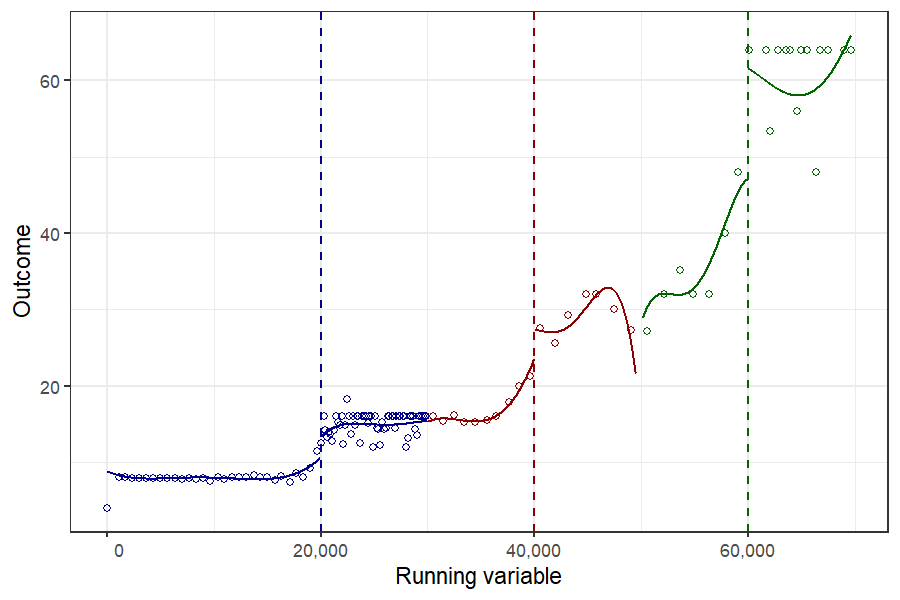
\includegraphics{artigo1_files/figure-latex/discontinuity-1.png}
\caption{Discontinuity in Backhaul program velocity by population
cut-offs: 20,000; 40,000; 60,000 \label{fig:2}}
\end{figure}

The McCrary manipulation test of cutoffs (McCrary 2008) looks if there
is a selection into treatment, analysing the density distribution of the
running variable around the cutoff. An alternative test was developed by
Cattaneo \emph{et al.} (2019) and Cattaneo \emph{et al.} (2020), where
confidence bands are provided, well suited for RDD designs. Results for
this test are presented in Table \ref{tab:test_tab} Figure
\ref{fig:test_plot} for all three cutoffs.

\begin{table}[H]

\caption{\label{tab:test_tab}Cattaneo, Jansson and Ma manipulation test of cutoffs}
\centering
\resizebox{\linewidth}{!}{
\begin{tabu} to \linewidth {>{\raggedleft}X>{\raggedleft}X>{\raggedleft}X>{\raggedleft}X>{\raggedleft}X>{\raggedleft\arraybackslash}p{3cm}>{\raggedleft}X}
\toprule
Cutoff & Bw & N & Nl & Nr & T (jackknife) & P.value\\
\midrule
20,000 & 3,285 & 3,001 & 227 & 145 & 0.265 & 0.791\\
40,000 & 3,201 & 226 & 42 & 27 & -0.717 & 0.473\\
60,000 & 9,440 & 115 & 44 & 26 & -1.640 & 0.101\\
\bottomrule
\multicolumn{7}{l}{\rule{0pt}{1em}Obs.1: Optimum bandwidht selection following Imbens \& Kalyanaraman (2012).}\\
\multicolumn{7}{l}{\rule{0pt}{1em}Obs.2: Unrestricted density estimation, triangular Kernel and VCE by jackknife.}\\
\multicolumn{7}{l}{\rule{0pt}{1em}Obs.3: Bw=bandwidth; N, Nl and Nr are total n\# of obs., n\# on the left and n\# on the right.}\\
\end{tabu}}
\end{table}

\begin{figure}
\centering
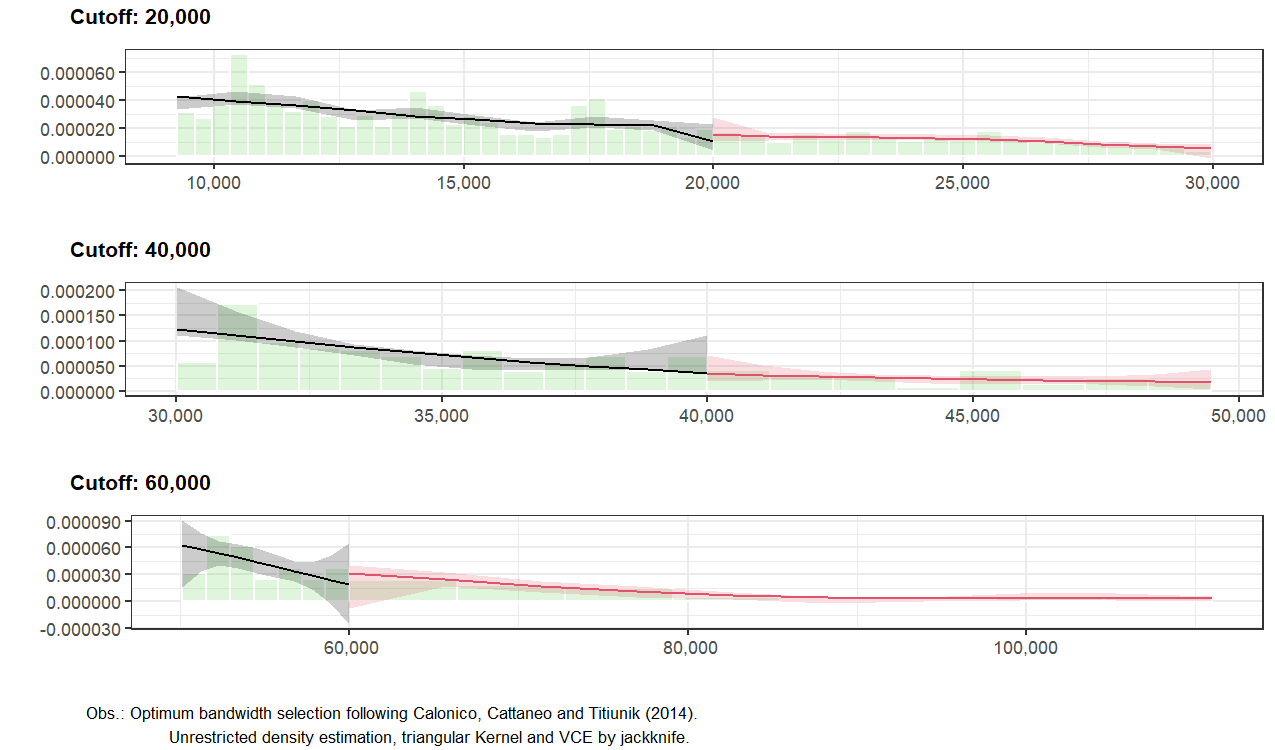
\includegraphics{artigo1_files/figure-latex/test_plot-1.png}
\caption{Density plot - Cattaneo, Jansson and Ma manipulation test of
cutoffs \label{fig:test_plot}}
\end{figure}

The manipulation test suggests that our identification strategy is
valid, for all three cutoffs, although the last one in a lower
significant level, the cutoff with a lower number of observations. As we
can see on Figure \ref{fig:test_plot}, the visual inspect confirms the
test results. However, Brazil has an odd population distribution, with
unexpected jumps in some population ranges. Monasterio (2013) shows that
these jumps occurs due to a legislation regarding Federal transfers of
resources to municipalities (\emph{Fundo de Participação dos Municípios
- FPM}), based on the population size.\footnote{According to the
  Decree-Law 1,881/1981, there are 17 ranges of population, with
  increasing resources being distributed for each range. The cuts are:
  10,188; 13,584; 16,980; 23,772; 30,564; 37,356; 44,148; 50,940;
  61,128; 71,316; 81,504; 91,692; 101,880; 115,464; 129,048; 142,632;
  156,216. Available in
  \url{http://www.planalto.gov.br/ccivil_03/Decreto-Lei/1965-1988/Del1881.htm}}.
Despite there are no intersections of Backhaul and FPM's cutoffs, we
control for the later one, in order to avoid any confounder effect
regarding this situation in results.

\hypertarget{descriptive-statistics}{%
\subsection{Descriptive statistics}\label{descriptive-statistics}}

Despite these clear discontinuities, a set of covariates were collected,
in order to control for any further confounders that might remain. Lack
of information at municipal level is one of the weakness in Brazilian
researches at this territory level. Census occurs only every ten years,
remaining just few administrative data in the between years, some of
them with low quality (mainly for small cities). Even tough, considering
that this is the only source of the main socioeconomic variables, we use
information from the last two censuses (2000 and 2010), organized by
Brazilian Institute of Statistics and Geography (IBGE). Also from IBGE,
we collect total population estimates and GDP. Considering that direct
cash transfers are important in Brazil, we collect data from the two
major programs: Bolsa Família (PBF) and Benefício de Prestação
Continuada for elders (BPC), booth organized by Ministry of
Citizenship\footnote{PBF is one of the biggest conditional cash transfer
  program in the world. The target are families under the extreme
  poverty and poverty lines (in 2020, families earning up to R\$ 89 by
  person, or U\$ 15, by month are considered extremely poor, while
  families above that amount and up to R\$ 178, or U\$ 31, are
  considered poor), focused one children. As counter part, school
  attendance and vaccination are required. PBF reaches around 14 million
  families in Brazil in 2020. On the other hand, BPC is a program for
  elderly and handicapped. The poor population in this profile (people
  aged 65 or over and all handicapped) are eligible for a minimum wage
  paycheck.}. In addition, we collect the mass of wages (formal labour
market) from RAIS database, organized by Ministry of Economy\footnote{In
  Brazil, every formal company have to fill the Annual Relation of
  Social Information (RAIS), with the profile of all workers they had in
  the calendar year, including wages.}. We also collected information
from National Institute of Meteorology, to control for rain and
temperature in election day, following Fujiwara \emph{et al.} (2016).
Municipalities were joined by the nearest distance between the center of
the city and the closest meteorological station.

In addition, we collected data from Ministry of Health regarding
homicide and suicide, but, due to poor quality of data (missing values),
we had to discard them. Public finance data were collected too, but
discarded due to missing problem and for being highly correlated with
other covariates (like GDP and population). In fact, some of covariates
were discarded due to high correlation (for example electricity, car and
computer ownership). Finally, we collected fiscal data, from Ministry of
Economy, regarding public expenses (current expenses and investments),
but again due to missing data and high correlation with other covariates
(like GDP and mass of wages) these variables were dropped too.

\begin{table}[H]

\caption{\label{tab:variables}Description of varibles by type and source}
\centering
\fontsize{9}{11}\selectfont
\begin{tabu} to \linewidth {>{\raggedright\arraybackslash}p{1.5cm}>{\raggedright\arraybackslash}p{3.5cm}>{\raggedright}X>{\raggedright\arraybackslash}p{2.5cm}}
\toprule
Category & Variable & Description & Source\\
\midrule
 & Turnout & Participation percentage of total electorate & TSE\\

 & Vote share & Vote share of parties and/or orientation of parties (left, center or right) & TSE\\

 & Blank and null votes & Percentage of blank and null votes in total & TSE\\

\multirow{-4}{1.5cm}{\raggedright\arraybackslash Outcome} & Donations & Declared donation received for campaign purpose & TSE\\
\cmidrule{1-4}
Running & Population & Estimated population & IBGE\\
\cmidrule{1-4}
 & Black & Percentage of blacks in population & IBGE\\

 & College & Percentage of people with college degree & IBGE\\

 & Married & Percetage of people married & IBGE\\

 & Income & Median household income & IBGE\\

 & Population over 60 years & Percentage of population over 60 years in population & IBGE\\

 & Radio & Percentage of households with radio & IBGE\\

 & Rural & Percentage of population in rural areas & IBGE\\

 & Television & Percentage of households with television & IBGE\\

 & Working age population & Percentage of population in working age & IBGE\\

 & GDP & Gross Domestic Product & IBGE\\

 & BPC & Ratio of BPC payments and GDP & MC and IBGE\\

 & PBF & Ratio of PBF payments and GDP & MC and IBGE\\

 & Formal wage & Ratio of formal wages (sum) and GDP & ME and IBGE\\

 & Temperature & Average temperature a week before and after election day & Inmet\\

 & Rain & Rain preciptation in election day & Inmet\\

\multirow{-16}{1.5cm}{\raggedright\arraybackslash Controls} & Fibra-optic & Fibra-optic internet infrasctructure in municipality & Anatel\\
\bottomrule
\multicolumn{4}{l}{\rule{0pt}{1em}Source: IBGE, Inmet, ME (Ministry of Economy), MC (Ministry of Citizenship) and Anatel.}\\
\end{tabu}
\end{table}

Outcomes are election results, organized by Superior Election Court
(TSE)\footnote{\emph{Tribunal Superior Eleitoral} in Portuguese.}. We
will analyze 2008, 2010 and 2012 elections, covering two municipal and
one national suffrage. The main outcomes we will analyze are: turnout,
percentage of blank or null votes\footnote{In Brazilian election, people
  may put a blank vote, which are not computed for any candidate and is
  not considered for official results, as well null votes. The
  difference consists in the way the registration of these votes are
  made: the blank vote is available as a button in the electronic
  ballot, while the null vote occurs when someone enters an invalid
  candidate number into the ballot and confirms the vote.} and vote
shares, for left wing, center or right wing parties (following Power \&
Zucco Jr (2012) and the party index from Brazilian Legislative
Survey\footnote{Version 7, available in
  \url{https://dataverse.harvard.edu/dataverse/bls;jsessionid=992eedb7e954a17ef718c7078cf5?widget=dataverse\%40harvard\&q=\&types=dataverses\%3Afiles\%3Adatasets\&sort=dateSort\&order=desc\&page=3}}.
Left wing parties are those up to quantile 0.25 of the party index,
center parties are those between 0.25 and 0.75 and right wing parties
are those above).

Descriptive statistics are separated by year (2008, 2010 and 2012),
considering 2000 Census data for 2008 statistics and 2010 Census for
2010 and 2012. All the other variables refers to the respective year.

\begin{table}[H]

\caption{\label{tab:desc.2008}Descriptive statistics by population size of municipality, 2008}
\centering
\begin{tabu} to \linewidth {>{\raggedright\arraybackslash}p{4cm}>{\raggedright}X>{\raggedright}X>{\raggedright}X>{\raggedright}X}
\toprule
Variable & Under 20k & Above 20k to 40k & Above 40k to 60k & Above 60k\\
\midrule
Avg. Temperature & 24.2 & 25.6 & 26.4 & 27.2\\
Black & 53.4 & 65.5 & 68.1 & 68.6\\
BPC & 0.3 & 0.8 & 0.8 & 0.9\\
College & 0.7 & 0.6 & 0.6 & 0.8\\
Fiber-optic & 23.1 & 34.2 & 33.6 & 47.2\\
Formal Wages & 11.5 & 11.5 & 12.8 & 13.8\\
GDP & 57,285 & 187,775 & 306,319 & 856,740\\
Married & 30 & 24.1 & 22 & 22.5\\
Median Income & 603.2 & 549.6 & 555.2 & 645.2\\
PBF & 2.5 & 3 & 2.6 & 2\\
Pop. over 60 years & 9.9 & 8.5 & 8 & 7\\
Population & 8,042 & 27,272 & 47,976 & 97,096\\
Radio & 79.3 & 75.4 & 75.6 & 76.1\\
Rain (elect. day) & 3.3 & 1.7 & 1.9 & 2.9\\
Rural & 49.8 & 46.6 & 40.3 & 32.2\\
Television & 69.2 & 66.4 & 68.1 & 73.6\\
Working Pop. & 41.4 & 38.8 & 37.9 & 38.9\\
Observations & 2,733 & 520 & 107 & 72\\
\bottomrule
\multicolumn{5}{l}{\rule{0pt}{1em}Source: IBGE, Inmet, ME, MC and Anatel.}\\
\end{tabu}
\end{table}

All three tables show a high heterogeneity in Brazil. Regional
inequalities, as pointed before, are particularly important and should
be considered in standard error estimates. It is very likely that
municipalities in the northeast and in the south regions show different
behavior that may possibly affect error distributions, that should be
addressed by, for example, clustered standard errors, strategy we adopt
here.

In order to clarify identification validity, Table \ref{tab:t.test}
presents a simple t-test for 20,000 population with a 5,000 people
(adhoc) cutoff. Since this is the cutoff with larger sample size,
results should be more robust.

\begin{table}[H]

\caption{\label{tab:t.test}Covariates means difference test for 20,000 cutoff, 2008, 2010 and 2012}
\centering
\begin{tabu} to \linewidth {>{\raggedright}X>{\raggedright}X>{\raggedright}X>{\raggedright}X}
\toprule
Var & Diff 2008 & Diff 2010 & Diff 2012\\
\midrule
renda\_med\_2000 & 15.3 & -88.0*** & -47.7*\\
60\_anos\_2000 & 0.02 & 0.02 & 0.17\\
rural\_2000 & 3.56* & 7.26*** & 5.35***\\
negro\_2000 & -2.25 & 2.29* & 0.66\\
radio\_2000 & -0.33 & -1.57* & -0.54\\
televisao\_2000 & -1.81 & -2.34*** & -1.67**\\
ens\_sup\_2000 & 0.07 & -0.28** & -0.17*\\
casado\_2000 & 0.52 & -0.07 & 0.19\\
pea\_2000 & -0.14 & -2.25*** & -0.89\\
PRECIP\_DIA & 0.0 & 0.3 & 0.1\\
TEMP\_MED & -0.1 & 0.2 & 0.3\\
valor\_bolsa & 0.19 & 0.68*** & 0.55**\\
valor\_bpc\_idoso & -0.23** & -0.25*** & -0.15\\
PIB & -7,108.4 & -74,974.7** & -91,131.7*\\
salarios\_rais & -1.30*** & -1.35* & -0.99\\
fibra & -8.71** & -6.22 & -5.32\\
\bottomrule
\multicolumn{4}{l}{\rule{0pt}{1em}Source: IBGE, Inmet, ME, MC and Anatel.}\\
\multicolumn{4}{l}{\rule{0pt}{1em}Obs.1: Null hypotheses is no difference.}\\
\multicolumn{4}{l}{\rule{0pt}{1em}Obs.2: * = significant at 10\%; ** = significant at 5\%; *** = significant at 1\%.}\\
\multicolumn{4}{l}{\rule{0pt}{1em}Obs.3: Bandwidth: 3,500}\\
\end{tabu}
\end{table}

Results for 2008 year in Table \ref{tab:t.test} (which, indeed, refers
to 2000 census for socioeconomic variables) show that there were no
significant differences for most of the characteristics between
municipalities just above and just below the cut-off, except for the
population (and velocity), as expected. Some results, however, do not
hold in 2010 and 2012, years with values collected from 2010 census and,
hence, closer to the years of analysis. Some covariates, like formal
wages and BPC seems to be different across municipalities, while other
covariates changes its significance in 2010 and 2012 samples. Overall,
Table \ref{tab:t.test} results suggests that our identification strategy
should work, if controlled for some covariates, and even more if applied
to a narrow cutoff (which will be the case).

\hypertarget{results}{%
\section{Results}\label{results}}

We begin our analysis of results looking the effects of broadband in
participation. Considering that there are two rounds for two types of
offices, mayor and president, and some municipalities might not have a
second round, we focus only in the first one, using, hence, the larger
sample size as possible.

Results in Table \ref{tab:reg.part} suggest no relationship between
broadband internet and participation in elections. For all regressions,
considering the three cutoffs, and pooled results, only two showed
significant relationship. Since participation in elections is mandatory
in Brazil, and turnout is relatively high (around 80\%), there is no
much room to improve this situation. These results are in line with
Menezes (2015) for Brazil, as well as results reported by Miner (2015)
for Malaysia, but differs from results reported in USA and European
countries (Jaber 2013; Falck \emph{et al.} 2014; Gavazza \emph{et al.}
2015; Campante \emph{et al.} 2017). Another way to look to this
relationship is the difference in turnout between elections, presented
in Table \ref{tab:reg.part.dif}.

\begin{table}[H]

\caption{\label{tab:reg.part}RDD regression results for turnout. Election years: 2008, 2010 and 2012. Brazil}
\centering
\begin{tabular}[t]{lllrrrrrr}
\toprule
Year & Cutoff & Type & Bw & Obs. & Estimates & SE & p.value & Weight\\
\midrule
 &  & With covariates & 3,285 & 380 & 0.001 & 0.002 & 0.608 & 0.814\\


 & \multirow{-2}{*}{\raggedright\arraybackslash 20000} & Without covariates & 3,285 & 380 & 0.002 & 0.002 & 0.225 & 0.814\\


 &  & With covariates & 3,201 & 58 & 0.006 & 0.005 & 0.268 & 0.138\\


 & \multirow{-2}{*}{\raggedright\arraybackslash 40000} & Without covariates & 3,201 & 58 & 0.002 & 0.001 & 0.001 & 0.138\\


 &  & With covariates & 9,440 & 67 & -0.001 & 0.001 & 0.248 & 0.049\\


 & \multirow{-2}{*}{\raggedright\arraybackslash 60000} & Without covariates & 9,440 & 67 & -0.004 & 0.004 & 0.377 & 0.049\\


 &  & With covariates & 5,930 & 847 & 0.000 & 0.000 & 0.568 & 1.000\\


\multirow{-8}{*}{\raggedright\arraybackslash 2008} & \multirow{-2}{*}{\raggedright\arraybackslash Pooled} & Without covariates & 5,593 & 783 & 0.000 & 0.000 & 0.439 & 1.000\\

\cmidrule{1-9}
 &  & With covariates & 2,939 & 352 & -0.004 & 0.006 & 0.438 & 0.815\\


 & \multirow{-2}{*}{\raggedright\arraybackslash 20000} & Without covariates & 2,939 & 352 & 0.007 & 0.007 & 0.267 & 0.815\\


 &  & With covariates & 3,769 & 79 & 0.010 & 0.028 & 0.711 & 0.138\\


 & \multirow{-2}{*}{\raggedright\arraybackslash 40000} & Without covariates & 3,769 & 79 & -0.001 & 0.004 & 0.880 & 0.138\\


 &  & With covariates & 7,547 & 58 & 0.009 & 0.009 & 0.313 & 0.047\\


 & \multirow{-2}{*}{\raggedright\arraybackslash 60000} & Without covariates & 7,547 & 58 & 0.003 & 0.003 & 0.216 & 0.047\\


 &  & With covariates & 4,032 & 568 & -0.018 & 0.004 & 0.903 & 1.000\\


\multirow{-8}{*}{\raggedright\arraybackslash 2010} & \multirow{-2}{*}{\raggedright\arraybackslash Pooled} & Without covariates & 3,225 & 464 & -0.011 & 0.001 & 0.841 & 1.000\\

\cmidrule{1-9}
 &  & With covariates & 2,133 & 224 & 0.023 & 0.007 & 0.002 & 0.796\\


 & \multirow{-2}{*}{\raggedright\arraybackslash 20000} & Without covariates & 2,133 & 224 & 0.446 & 6.514 & 0.945 & 0.796\\


 &  & With covariates & 3,749 & 76 & 0.003 & 0.002 & 0.201 & 0.159\\


 & \multirow{-2}{*}{\raggedright\arraybackslash 40000} & Without covariates & 3,749 & 76 & -0.004 & 0.008 & 0.568 & 0.159\\


 &  & With covariates & 7,622 & 65 & -0.004 & 0.006 & 0.479 & 0.045\\


 & \multirow{-2}{*}{\raggedright\arraybackslash 60000} & Without covariates & 7,622 & 65 & -0.001 & 0.001 & 0.464 & 0.045\\


 &  & With covariates & 2,753 & 394 & -0.005 & 0.000 & 0.368 & 1.000\\


\multirow{-8}{*}{\raggedright\arraybackslash 2012} & \multirow{-2}{*}{\raggedright\arraybackslash Pooled} & Without covariates & 2,781 & 397 & -0.006 & 0.000 & 0.433 & 1.000\\
\bottomrule
\multicolumn{9}{l}{\rule{0pt}{1em}Standard Errors are clustered by regions}\\
\multicolumn{9}{l}{\rule{0pt}{1em}Turnout for first round}\\
\multicolumn{9}{l}{\rule{0pt}{1em}Bw=bandwidth}\\
\multicolumn{9}{l}{\rule{0pt}{1em}LATE estimates.}\\
\end{tabular}
\end{table}

Results suggests that broadband did not changed turnout rate between
elections in Brazil. It is an interesting result since a new possibility
of leisure, at least apparently, did not reduce people participation in
elections. However, in another backgrounds, where participation in
elections are not mandatory, results may be different (like in Germany
and UK, showed by Falck \emph{et al.} (2014) and Gavazza \emph{et al.}
(2015), respectively).

\begin{table}[H]

\caption{\label{tab:reg.part.dif}RDD regression results for difference in turnout. Election years: 2008, 2010 and 2012}
\centering
\begin{tabular}[t]{lllrrrrrr}
\toprule
Year & Cutoff & Type & Bw & Obs. & Estimates & SE & p.value & Weight\\
\midrule
 &  & With covariates & 3,921 & 389 & -0.002 & 0.002 & 0.244 & 0.890\\


 & \multirow{-2}{*}{\raggedright\arraybackslash 20000} & Without covariates & 3,921 & 389 & -0.004 & 0.005 & 0.456 & 0.890\\


 &  & With covariates & 3,418 & 63 & -0.001 & 0.003 & 0.737 & 0.159\\


 & \multirow{-2}{*}{\raggedright\arraybackslash 40000} & Without covariates & 3,418 & 63 & 0.001 & 0.001 & 0.288 & 0.159\\


 &  & With covariates & 11,298 & 71 & -0.001 & 0.000 & 0.186 & 0.052\\


 & \multirow{-2}{*}{\raggedright\arraybackslash 60000} & Without covariates & 11,298 & 71 & -0.004 & 0.003 & 0.105 & 0.052\\


 &  & With covariates & 8,037 & 1,073 & 0.002 & 0.000 & 0.323 & 1.000\\


\multirow{-8}{*}{\raggedright\arraybackslash 2008} & \multirow{-2}{*}{\raggedright\arraybackslash Pooled} & Without covariates & 8,085 & 1,079 & 0.002 & 0.000 & 0.341 & 1.000\\

\cmidrule{1-9}
 &  & With covariates & 3,787 & 436 & -0.001 & 0.003 & 0.612 & 0.796\\


 & \multirow{-2}{*}{\raggedright\arraybackslash 20000} & Without covariates & 3,787 & 436 & 0.003 & 0.002 & 0.097 & 0.796\\


 &  & With covariates & 3,170 & 63 & 0.005 & 0.014 & 0.748 & 0.150\\


 & \multirow{-2}{*}{\raggedright\arraybackslash 40000} & Without covariates & 3,170 & 63 & 0.001 & 0.006 & 0.894 & 0.150\\


 &  & With covariates & 6,268 & 46 & -0.003 & 0.001 & 0.000 & 0.054\\


 & \multirow{-2}{*}{\raggedright\arraybackslash 60000} & Without covariates & 6,268 & 46 & 0.005 & 0.005 & 0.350 & 0.054\\


 &  & With covariates & 5,807 & 856 & 0.006 & 0.000 & 0.579 & 1.000\\


\multirow{-8}{*}{\raggedright\arraybackslash 2010} & \multirow{-2}{*}{\raggedright\arraybackslash Pooled} & Without covariates & 4,814 & 681 & 0.011 & 0.004 & 0.553 & 1.000\\

\cmidrule{1-9}
 &  & With covariates & 4,285 & 464 & 0.003 & 0.001 & 0.020 & 0.822\\


 & \multirow{-2}{*}{\raggedright\arraybackslash 20000} & Without covariates & 4,285 & 464 & 0.004 & 0.002 & 0.049 & 0.822\\


 &  & With covariates & 3,911 & 75 & 0.006 & 0.005 & 0.233 & 0.155\\


 & \multirow{-2}{*}{\raggedright\arraybackslash 40000} & Without covariates & 3,911 & 75 & -0.001 & 0.002 & 0.648 & 0.155\\


 &  & With covariates & 9,312 & 79 & -0.004 & 0.013 & 0.753 & 0.055\\


 & \multirow{-2}{*}{\raggedright\arraybackslash 60000} & Without covariates & 9,312 & 79 & -0.003 & 0.005 & 0.572 & 0.055\\


 &  & With covariates & 3,950 & 526 & -0.002 & 0.000 & 0.831 & 1.000\\


\multirow{-8}{*}{\raggedright\arraybackslash 2012} & \multirow{-2}{*}{\raggedright\arraybackslash Pooled} & Without covariates & 3,908 & 523 & -0.002 & 0.000 & 0.899 & 1.000\\
\bottomrule
\multicolumn{9}{l}{\rule{0pt}{1em}Standard Errors are clustered by regions}\\
\multicolumn{9}{l}{\rule{0pt}{1em}Turnout for first round}\\
\multicolumn{9}{l}{\rule{0pt}{1em}Bw=bandwidth}\\
\multicolumn{9}{l}{\rule{0pt}{1em}LATE estimates.}\\
\end{tabular}
\end{table}

The next outcome regards to the percentage of blank or null votes (Table
\ref{tab:r.pct.bn}). Again, there is little support in favor of the
influence of broadband internet in blank or null votes (a \emph{proxy}
for ``absence of engagement with political process'', since these votes
can be seen as a ``whatever vote''). So, results so far suggests that
broadband did not encourage or discourage people to turnout neither
people to place more directed votes in elections (again in accordance to
Menezes (2015) results).

\begin{table}[H]

\caption{\label{tab:r.pct.bn}RDD regression results for blank of null votes. Election years: 2008, 2010 and 2012}
\centering
\begin{tabular}[t]{lllrrrrrr}
\toprule
Year & Cutoff & Type & Bw & Obs. & Estimates & SE & p.value & Weight\\
\midrule
 &  & With covariates & 3,624 & 212 & 0.009 & 0.013 & 0.465 & 0.781\\


 & \multirow{-2}{*}{\raggedright\arraybackslash 20000} & Without covariates & 3,624 & 212 & -0.016 & 0.055 & 0.771 & 0.781\\


 &  & With covariates & 3,171 & 40 & 0.014 & 0.031 & 0.663 & 0.167\\


 & \multirow{-2}{*}{\raggedright\arraybackslash 40000} & Without covariates & 3,171 & 40 & 0.000 & 0.004 & 0.967 & 0.167\\


 &  & With covariates & 13,386 & 58 & -0.009 & 0.022 & 0.676 & 0.052\\


 & \multirow{-2}{*}{\raggedright\arraybackslash 60000} & Without covariates & 13,386 & 58 & 0.001 & 0.008 & 0.856 & 0.052\\


 &  & With covariates & 5,064 & 384 & 0.000 & 0.000 & 0.918 & 1.000\\


\multirow{-8}{*}{\raggedright\arraybackslash 2008} & \multirow{-2}{*}{\raggedright\arraybackslash Pooled} & Without covariates & 5,293 & 401 & 0.000 & 0.000 & 0.879 & 1.000\\

\cmidrule{1-9}
 &  & With covariates & 3,341 & 389 & 0.004 & 0.002 & 0.088 & 0.802\\


 & \multirow{-2}{*}{\raggedright\arraybackslash 20000} & Without covariates & 3,341 & 389 & -0.004 & 0.002 & 0.011 & 0.802\\


 &  & With covariates & 3,682 & 74 & -0.001 & 0.002 & 0.652 & 0.148\\


 & \multirow{-2}{*}{\raggedright\arraybackslash 40000} & Without covariates & 3,682 & 74 & 0.000 & 0.005 & 0.962 & 0.148\\


 &  & With covariates & 8,379 & 65 & 0.000 & 0.000 & 0.833 & 0.050\\


 & \multirow{-2}{*}{\raggedright\arraybackslash 60000} & Without covariates & 8,379 & 65 & 0.000 & 0.001 & 0.845 & 0.050\\


 &  & With covariates & 5,812 & 858 & -0.005 & 0.000 & 0.409 & 1.000\\


\multirow{-8}{*}{\raggedright\arraybackslash 2010} & \multirow{-2}{*}{\raggedright\arraybackslash Pooled} & Without covariates & 4,262 & 595 & 0.066 & 2.042 & 0.696 & 1.000\\

\cmidrule{1-9}
 &  & With covariates & 2,529 & 163 & 1.659 & 91.191 & 0.985 & 0.772\\


 & \multirow{-2}{*}{\raggedright\arraybackslash 20000} & Without covariates & 2,529 & 163 & -0.020 & 0.028 & 0.472 & 0.772\\


 &  & With covariates & 3,304 & 47 & 0.015 & 0.011 & 0.186 & 0.162\\


 & \multirow{-2}{*}{\raggedright\arraybackslash 40000} & Without covariates & 3,304 & 47 & 0.018 & 0.018 & 0.315 & 0.162\\


 &  & With covariates & 12,260 & 72 & 0.211 & 4.966 & 0.966 & 0.066\\


 & \multirow{-2}{*}{\raggedright\arraybackslash 60000} & Without covariates & 12,260 & 72 & -0.124 & 1.543 & 0.936 & 0.066\\


 &  & With covariates & 3,556 & 299 & 0.003 & 0.000 & 0.676 & 1.000\\


\multirow{-8}{*}{\raggedright\arraybackslash 2012} & \multirow{-2}{*}{\raggedright\arraybackslash Pooled} & Without covariates & 3,611 & 302 & 0.003 & 0.000 & 0.685 & 1.000\\
\bottomrule
\multicolumn{9}{l}{\rule{0pt}{1em}Standard Errors are clustered by regions.}\\
\multicolumn{9}{l}{\rule{0pt}{1em}For mayor elections (2008 and 2012) and presidential election (2010).}\\
\multicolumn{9}{l}{\rule{0pt}{1em}Bw=bandwidth.}\\
\multicolumn{9}{l}{\rule{0pt}{1em}LATE estimates.}\\
\end{tabular}
\end{table}

No huge changes are observed when we look to the differences in these
percentages between elections (Table \ref{tab:r.pct.bn.dif}).

\begin{table}[H]

\caption{\label{tab:r.pct.bn.dif}RDD regression results for difference in blank of null votes. Election years: 2008, 2010 and 2012}
\centering
\begin{tabular}[t]{lllrrrrrr}
\toprule
Year & Cutoff & Type & Bw & Obs. & Estimates & SE & p.value & Weight\\
\midrule
 &  & With covariates & 3,967 & 117 & 0.016 & 0.013 & 0.211 & 0.753\\


 & \multirow{-2}{*}{\raggedright\arraybackslash 20000} & Without covariates & 3,967 & 117 & -0.112 & 1.073 & 0.917 & 0.753\\


 &  & With covariates & 3,767 & 32 & 0.005 & 0.003 & 0.149 & 0.191\\


 & \multirow{-2}{*}{\raggedright\arraybackslash 40000} & Without covariates & 3,767 & 32 & 0.001 & 0.001 & 0.062 & 0.191\\


 &  & With covariates & 25,181 & 82 & -0.001 & 0.001 & 0.568 & 0.057\\


 & \multirow{-2}{*}{\raggedright\arraybackslash 60000} & Without covariates & 25,181 & 82 & -0.001 & 0.001 & 0.325 & 0.057\\


 &  & With covariates & 4,721 & 194 & 0.002 & 0.000 & 0.594 & 1.000\\


\multirow{-8}{*}{\raggedright\arraybackslash 2008} & \multirow{-2}{*}{\raggedright\arraybackslash Pooled} & Without covariates & 6,803 & 299 & 0.001 & 0.000 & 0.796 & 1.000\\

\cmidrule{1-9}
 &  & With covariates & 3,727 & 428 & 0.002 & 0.002 & 0.196 & 0.798\\


 & \multirow{-2}{*}{\raggedright\arraybackslash 20000} & Without covariates & 3,727 & 428 & 0.001 & 0.002 & 0.508 & 0.798\\


 &  & With covariates & 3,433 & 67 & -0.001 & 0.003 & 0.771 & 0.149\\


 & \multirow{-2}{*}{\raggedright\arraybackslash 40000} & Without covariates & 3,433 & 67 & -0.002 & 0.007 & 0.745 & 0.149\\


 &  & With covariates & 9,434 & 70 & 0.001 & 0.000 & 0.002 & 0.053\\


 & \multirow{-2}{*}{\raggedright\arraybackslash 60000} & Without covariates & 9,434 & 70 & 0.000 & 0.000 & 0.000 & 0.053\\


 &  & With covariates & 7,162 & 1,065 & 0.001 & 0.000 & 0.257 & 1.000\\


\multirow{-8}{*}{\raggedright\arraybackslash 2010} & \multirow{-2}{*}{\raggedright\arraybackslash Pooled} & Without covariates & 5,313 & 774 & 0.005 & 0.000 & 0.268 & 1.000\\

\cmidrule{1-9}
 &  & With covariates & 2,633 & 124 & 0.108 & 0.226 & 0.633 & 0.759\\


 & \multirow{-2}{*}{\raggedright\arraybackslash 20000} & Without covariates & 2,633 & 124 & -0.243 & 1.203 & 0.840 & 0.759\\


 &  & With covariates & 2,721 & 38 & 0.014 & 0.012 & 0.226 & 0.181\\


 & \multirow{-2}{*}{\raggedright\arraybackslash 40000} & Without covariates & 2,721 & 38 & 0.023 & 0.015 & 0.135 & 0.181\\


 &  & With covariates & 15,880 & 78 & -0.085 & 0.714 & 0.906 & 0.060\\


 & \multirow{-2}{*}{\raggedright\arraybackslash 60000} & Without covariates & 15,880 & 78 & -0.026 & 0.051 & 0.613 & 0.060\\


 &  & With covariates & 8,256 & 607 & -0.013 & 0.002 & 0.572 & 1.000\\


\multirow{-8}{*}{\raggedright\arraybackslash 2012} & \multirow{-2}{*}{\raggedright\arraybackslash Pooled} & Without covariates & 6,084 & 432 & 0.004 & 0.001 & 0.786 & 1.000\\
\bottomrule
\multicolumn{9}{l}{\rule{0pt}{1em}Standard Errors are clustered by regions.}\\
\multicolumn{9}{l}{\rule{0pt}{1em}For mayor elections (2008 and 2012) and presidential election (2010).}\\
\multicolumn{9}{l}{\rule{0pt}{1em}Bw=bandwidth.}\\
\multicolumn{9}{l}{\rule{0pt}{1em}LATE estimates.}\\
\end{tabular}
\end{table}

In last presidential elections (2018), polarization was dramatic in
Brazil. Left versus Right debate was at the center of the presidential
run, with the last four times presidential winner party (the left wing
Workers Party -- PT) being the main target. In fact, 2014 elections was
one of the closest seen in Brazil, when Mrs.~Rouseff defeated Mr.~Neves
(from central right Brazilian Social Democracy Party -- PSDB) with only
51.64\% of the valid votes in the second round. Internet may had a
important role in this scenario, since, back in 2010, Mr.~Lula da Silva,
the first president of Workers Party, had 80\% of presidency approval,
the highest value ever recorded.\footnote{A news about these figures are
  available in:
  \url{http://g1.globo.com/politica/noticia/2010/12/popularidade-de-lula-bate-recorde-e-chega-87-diz-ibope.html}}

Hence, a closer look at the relationship between broadband and vote
share of left parties since 2008 might shed light into this turnaround
in Brazil. As pointed before, vote shares were classified as left,
center or right based on Power \& Zucco Jr (2012) party index. Table
\ref{tab:parties} presents this organization.

Results suggests, once again, that there is no clear relationship
between broadband internet and the vote received by left wing parties in
elections for mayors and president (Table \ref{tab:r.pct.vote}). So,
unlike results reported by previous studies, there is little evidence of
important effects of internet on vote shares, at least when fixed
broadband is considered (Jaber 2013; Falck \emph{et al.} 2014; Gavazza
\emph{et al.} 2015; Campante \emph{et al.} 2017).

\begin{table}[H]

\caption{\label{tab:r.pct.vote}RDD regression for left wing parties vote share. Election years: 2008, 2010 and 2012}
\centering
\begin{tabular}[t]{lllrrrrrr}
\toprule
Year & Cutoff & Type & Bw & Obs. & Estimates & SE & p.value & Weight\\
\midrule
 &  & With covariates & 3,661 & 212 & -0.043 & 0.035 & 0.223 & 0.785\\


 & \multirow{-2}{*}{\raggedright\arraybackslash 20000} & Without covariates & 3,661 & 212 & -0.126 & 0.297 & 0.670 & 0.785\\


 &  & With covariates & 3,597 & 48 & 0.017 & 0.083 & 0.835 & 0.159\\


 & \multirow{-2}{*}{\raggedright\arraybackslash 40000} & Without covariates & 3,597 & 48 & 0.004 & 0.015 & 0.814 & 0.159\\


 &  & With covariates & 14,064 & 64 & 0.017 & 0.027 & 0.523 & 0.056\\


 & \multirow{-2}{*}{\raggedright\arraybackslash 60000} & Without covariates & 14,064 & 64 & 0.001 & 0.002 & 0.719 & 0.056\\


 &  & With covariates & 4,795 & 362 & 0.013 & 0.000 & 0.286 & 1.000\\


\multirow{-8}{*}{\raggedright\arraybackslash 2008} & \multirow{-2}{*}{\raggedright\arraybackslash Pooled} & Without covariates & 5,578 & 427 & 0.013 & 0.000 & 0.226 & 1.000\\

\cmidrule{1-9}
 &  & With covariates & 3,076 & 362 & 0.009 & 0.003 & 0.006 & 0.792\\


 & \multirow{-2}{*}{\raggedright\arraybackslash 20000} & Without covariates & 3,076 & 362 & -0.061 & 0.016 & 0.000 & 0.792\\


 &  & With covariates & 3,774 & 79 & -0.016 & 0.024 & 0.496 & 0.154\\


 & \multirow{-2}{*}{\raggedright\arraybackslash 40000} & Without covariates & 3,774 & 79 & 0.012 & 0.045 & 0.780 & 0.154\\


 &  & With covariates & 6,870 & 52 & 0.043 & 0.033 & 0.193 & 0.054\\


 & \multirow{-2}{*}{\raggedright\arraybackslash 60000} & Without covariates & 6,870 & 52 & -0.010 & 0.013 & 0.440 & 0.054\\


 &  & With covariates & 4,541 & 639 & 0.398 & 11.434 & 0.715 & 1.000\\


\multirow{-8}{*}{\raggedright\arraybackslash 2010} & \multirow{-2}{*}{\raggedright\arraybackslash Pooled} & Without covariates & 4,953 & 703 & -0.197 & 0.590 & 0.427 & 1.000\\

\cmidrule{1-9}
 &  & With covariates & 3,824 & 243 & -0.022 & 0.014 & 0.129 & 0.772\\


 & \multirow{-2}{*}{\raggedright\arraybackslash 20000} & Without covariates & 3,824 & 243 & -0.130 & 0.298 & 0.663 & 0.772\\


 &  & With covariates & 3,357 & 47 & -0.004 & 0.016 & 0.785 & 0.163\\


 & \multirow{-2}{*}{\raggedright\arraybackslash 40000} & Without covariates & 3,357 & 47 & 0.014 & 0.028 & 0.600 & 0.163\\


 &  & With covariates & 13,583 & 79 & -0.319 & 6.687 & 0.962 & 0.065\\


 & \multirow{-2}{*}{\raggedright\arraybackslash 60000} & Without covariates & 13,583 & 79 & -0.085 & 0.356 & 0.812 & 0.065\\


 &  & With covariates & 3,505 & 296 & 0.019 & 0.000 & 0.447 & 1.000\\


\multirow{-8}{*}{\raggedright\arraybackslash 2012} & \multirow{-2}{*}{\raggedright\arraybackslash Pooled} & Without covariates & 3,692 & 307 & 0.022 & 0.001 & 0.501 & 1.000\\
\bottomrule
\multicolumn{9}{l}{\rule{0pt}{1em}Standard Errors are clustered by regions.}\\
\multicolumn{9}{l}{\rule{0pt}{1em}For mayor elections (2008 and 2012) and presidential election (2010).}\\
\multicolumn{9}{l}{\rule{0pt}{1em}Left wing parties: PSTU, PSOL, PC do B, PT, PSB and PCO.}\\
\multicolumn{9}{l}{\rule{0pt}{1em}Bw=bandwidth.}\\
\multicolumn{9}{l}{\rule{0pt}{1em}LATE estimates.}\\
\end{tabular}
\end{table}

A limitation of RDD models is the bandwidth choice, that could influence
results. It is possible that a narrower or wider bandwidth give
different results, since fewer or more observations will be part of
regressions (trade off between randomness and precision). Considering
this possibility, Table \ref{tab:r.sig} presents only significant
results using also half or double bandwidths.

\begin{landscape}\begin{table}[!h]

\caption{\label{tab:r.sig}RDD regression with alternative bandwidths. Election years: 2008, 2010 and 2012}
\centering
\fontsize{9}{11}\selectfont
\begin{tabular}[t]{llllrrrrrl}
\toprule
Year & Model & Cutoff & Type & Bw & Obs. & Estimates & SE & p.value & Outcome\\
\midrule
 & Double-BW & 20000 & With covariates & 7,322 & 479 & -0.126 & 0.019 & 0.000 & Left Vote Share\\

 & LATE & 40000 & Without covariates & 3,201 & 58 & 0.002 & 0.001 & 0.001 & Turnout\\

 & Double-BW & 40000 & Without covariates & 6,401 & 128 & 0.005 & 0.001 & 0.001 & Turnout\\

 & Half-BW & 60000 & With covariates & 6,693 & 30 & -0.001 & 0.001 & 0.044 & Blank and Null\\

 & Double-BW & 60000 & With covariates & 28,129 & 163 & -0.003 & 0.001 & 0.019 & Left Vote Share\\

 & Half-BW & 60000 & With covariates & 4,720 & 29 & -0.001 & 0.000 & 0.000 & Turnout\\

 & Double-BW & 60000 & With covariates & 18,880 & 138 & -0.001 & 0.000 & 0.002 & Turnout\\

 & Double-BW & 60000 & Without covariates & 28,129 & 164 & -0.002 & 0.001 & 0.031 & Left Vote Share\\

\multirow{-9}{*}{\raggedright\arraybackslash 2008} & Double-BW & 60000 & Without covariates & 18,880 & 139 & -0.003 & 0.001 & 0.003 & Turnout\\
\cmidrule{1-10}
 & LATE & 20000 & With covariates & 3,341 & 389 & 0.004 & 0.002 & 0.088 & Blank and Null\\

 & Double-BW & 20000 & With covariates & 6,681 & 793 & 0.001 & 0.001 & 0.019 & Blank and Null\\

 & LATE & 20000 & With covariates & 3,076 & 362 & 0.009 & 0.003 & 0.006 & Left Vote Share\\

 & LATE & 20000 & Without covariates & 3,341 & 389 & -0.004 & 0.002 & 0.011 & Blank and Null\\

 & Double-BW & 20000 & Without covariates & 6,681 & 793 & -0.002 & 0.001 & 0.018 & Blank and Null\\

 & LATE & 20000 & Without covariates & 3,076 & 362 & -0.061 & 0.016 & 0.000 & Left Vote Share\\

 & Half-BW & 20000 & Without covariates & 1,538 & 184 & -0.083 & 0.027 & 0.002 & Left Vote Share\\

 & Double-BW & 20000 & Without covariates & 6,153 & 736 & -0.025 & 0.009 & 0.004 & Left Vote Share\\

 & Half-BW & 20000 & Without covariates & 1,470 & 176 & 0.027 & 0.010 & 0.006 & Turnout\\

 & Double-BW & 20000 & Without covariates & 5,879 & 709 & 0.004 & 0.002 & 0.100 & Turnout\\

 & Half-BW & 60000 & With covariates & 3,435 & 25 & 0.004 & 0.000 & 0.000 & Left Vote Share\\

\multirow{-12}{*}{\raggedright\arraybackslash 2010} & Half-BW & 60000 & With covariates & 3,774 & 25 & 0.000 & 0.000 & 0.001 & Turnout\\
\cmidrule{1-10}
 & LATE & 20000 & With covariates & 2,133 & 224 & 0.023 & 0.007 & 0.002 & Turnout\\

 & Double-BW & 20000 & With covariates & 4,266 & 475 & 0.008 & 0.004 & 0.023 & Turnout\\

 & Half-BW & 20000 & Without covariates & 1,265 & 73 & -0.006 & 0.002 & 0.013 & Blank and Null\\

 & Half-BW & 20000 & Without covariates & 1,912 & 116 & 0.058 & 0.028 & 0.039 & Left Vote Share\\

 & Half-BW & 20000 & Without covariates & 1,066 & 111 & -0.019 & 0.009 & 0.029 & Turnout\\

 & Double-BW & 40000 & With covariates & 6,607 & 96 & 0.019 & 0.010 & 0.065 & Blank and Null\\

 & Half-BW & 40000 & Without covariates & 1,652 & 25 & 0.034 & 0.009 & 0.000 & Blank and Null\\

 & Double-BW & 60000 & With covariates & 24,520 & 156 & -0.008 & 0.004 & 0.049 & Blank and Null\\

 & Half-BW & 60000 & With covariates & 3,811 & 27 & -0.005 & 0.002 & 0.003 & Turnout\\

 & Double-BW & 60000 & Without covariates & 24,520 & 156 & -0.007 & 0.002 & 0.001 & Blank and Null\\

\multirow{-11}{*}{\raggedright\arraybackslash 2012} & Double-BW & 60000 & Without covariates & 27,167 & 189 & -0.006 & 0.002 & 0.003 & Left Vote Share\\
\bottomrule
\multicolumn{10}{l}{\rule{0pt}{1em}Standard Errors are clustered by regions.}\\
\multicolumn{10}{l}{\rule{0pt}{1em}For mayor elections (2008 and 2012) and presidential election (2010).}\\
\multicolumn{10}{l}{\rule{0pt}{1em}Left wing parties: PSTU, PSOL, PC do B, PT, PSB and PCO.}\\
\multicolumn{10}{l}{\rule{0pt}{1em}Bw=bandwidth.}\\
\multicolumn{10}{l}{\rule{0pt}{1em}LATE estimates.}\\
\end{tabular}
\end{table}
\end{landscape}

With bandwidth doubled, a significant and negative effect of broadband
are observed for left wing vote share in 2008 (for the first and last
cutoffs). However, results are only significant with covariates, a
possible consequence due to the loss of randomness when the distance
from the cut-off increases. Turnout seems to be positively related to
broadband around 40,000 cut-off, while negatively related around 60,000,
this last one more robust to covariates and changes in the cut-off. This
is an interesting result, suggesting that cities with different sizes
may respond differently to the internet.

In 2010, negative relationship between broadband and left wing vote
shares seems to persist around 20,000 cutoff, although there is an
ambiguity in a specification with covariates, changing its sign in LATE
regression from positive to negative when covariates are omitted.
Considering that around the 60,000 cut-off results are positive with
covariate, these figures should be looked with even more caution.
Turnout shows a positive relationship only with half bandwidth, for
20,000 and 40,000 cutoffs, which don't seems to be a very robust results
because they are sensitive to covariates. Black and null percentage
votes are only significant for 20,000 cutoff, being highly sensitive to
covariates. Booth LATE and doubled bandwidth regression show a change in
sign when covariates are considered, putting in check the results.

Finally, left wing vote share is positively related in the first cut-off
and negatively related in the last one, but only without covariates.
Turnout shows a change of sign in the 20,000 cutoff when the bandwidth
is narrowed, making any conclusion problematic. Finally, blank and null
votes shows distinct behavior according to the cut-off, being negatively
related to broad band in the first and the last one, while positively
related in the middle.

Putting all these results together, it is hard to conclude that the
backhaul program, and, hence, broadband availability, made difference in
2008, 2010 and 2012 elections in terms of turnout, left wing vote share
and percentage of blank or null votes, at least when presidential and
mayor offices, and only the first round, area considered.\footnote{These
  are the natural scenarios to be first investigated because they are
  the more important offices in each election.} It may possible that
other offices present a different result. However, results (not
reported) are similar, with significance only for a negative
relationship between broadband and left wing vote share in municipal
chamber office election (\emph{vereador}), only for the first cut-off.
One more time, significant results are sparse, which means that it is
hard to point a consistent pattern linking broadband internet
availability to election outcomes. Finally, all polled regressions, a
general result regardless the cut-off, were not significant, reinforcing
this conclusion.

\hypertarget{discussion-and-conclusions}{%
\section{Discussion and conclusions}\label{discussion-and-conclusions}}

Relationship between broadband and elections outcome does not seems be
relevant in Brazil, at least when fixed broadband are considered,
neither for local or national elections. Despite our robust
identification strategy, we did not find strong relationship between
broadband availability, measured by the jumps of internet velocity in
the backhaul program roll out, and election outcomes (turnout,
percentage of blank and null votes and left parties vote share), in line
with finds reported by Menezes (2015), with a different approach, giving
robustness to our finds.

However, these results are different from those reported in some part of
the literature, mostly concentrated in European countries and USA (Jaber
2013; Falck \emph{et al.} 2014; Gavazza \emph{et al.} 2015; Campante
\emph{et al.} 2017), which could indicate that the background may be
important in this kind of analysis. First of all, vote is mandatory in
Brazil, which is not necessarily true in other countries. Second, the
political system in Brazil is presidentialist, in a federation republic,
which means that people may behavior differently than in a
parliamentarian system. Third, national congress deputies are elected by
proportional vote, while senators are elected by direct vote, situation
that may differ across countries. A fourth source of variation in
political background regards to the difference between unitary and
federal systems, that sets different rules to be played in the
``political game''.

Aside the political background, there is a qualification of internet
usage that is not addressed in our analysis. First of all, social
networks have grown in Brazil after 2010. WhatsApp, one of the most
popular social network in Brazil today, was created only in 2009, the
very same year internet campaign was regulated. Is it possible that,
today, mobile broadband and social medias usage in smartphones are more
important for communication and mobilization than older social medias
and connection made at home, through desktop or laptop computers.
Unfortunately, there is not available in Brazil the roll out of 3G and
4G technology implementation at municipality level, only at Direct
Dialling codes (DDDs)\footnote{The DDD codes are numbers that divides
  Brazil in 67 areas.}, which makes impossible to determine when the
technology begun to operate in every city\footnote{We contact the
  Regulation Agency of Telecommunication -- Anatel -- requesting mobile
  internet implementation at municipality level. Unfortunately, there is
  no such data base available.}.

Nonetheless, our paper contributes to bring into discussion that
internet and political outcomes should be viewed in a wider perspective,
meaning that some relationship may be circumstantial to idiosyncrasies
of the countries. Also, further investigation, like the role of the new
social medias and mobile broadband, are necessary to shed light in this
discussion, even because internet and social medias are still evolving.

\hypertarget{references}{%
\section*{References}\label{references}}
\addcontentsline{toc}{section}{References}

\hypertarget{refs}{}
\leavevmode\hypertarget{ref-aldrich_rational_1993}{}%
Aldrich, J.H. (1993). Rational choice and turnout. \emph{American
journal of political science}, 246--278.

\leavevmode\hypertarget{ref-ali_why_2013}{}%
Ali, S.N. \& Lin, C. (2013). Why people vote: Ethical motives and social
incentives. \emph{American economic Journal: microeconomics},
\textbf{5}, 73--98.

\leavevmode\hypertarget{ref-allcott_social_2017}{}%
Allcott, H. \& Gentzkow, M. (2017). Social media and fake news in the
2016 election. \emph{Journal of economic perspectives}, \textbf{31},
211--36.

\leavevmode\hypertarget{ref-anatel_relatorio_2010}{}%
Anatel. (2010). RELATÓRIO DE ACOMPANHAMENTO DAS METAS DE IMPLEMENTAÇÃO
DA INFRAESTRUTURA DE REDE DE SUPORTE DO STFC PARA CONEXÃO EM BANDA LARGA
(BACKHAUL).

\leavevmode\hypertarget{ref-banerjee_informed_2011}{}%
Banerjee, A., Kumar, S., Pande, R. \& Su, F. (2011). Do informed voters
make better choices? Experimental evidence from urban India.
\emph{Unpublished manuscript}. Retrieved June 4, 2017, from
\url{https://pdfs.semanticscholar.org/fc45/db4976c51fd67177757ca895896c3a01039e.pdf}

\leavevmode\hypertarget{ref-besley_handcuffs_2006}{}%
Besley, T. \& Prat, A. (2006). Handcuffs for the grabbing hand? Media
capture and government accountability. \emph{American economic review},
\textbf{96}, 720--736.

\leavevmode\hypertarget{ref-bimber_information_2003}{}%
Bimber, B. (2003). \emph{Information and American democracy: Technology
in the evolution of political power}. Cambridge University Press.

\leavevmode\hypertarget{ref-bimber_internet_1998}{}%
Bimber, B. (1998). The Internet and political mobilization: Research
note on the 1996 election season. \emph{Social Science Computer Review},
\textbf{16}, 391--401.

\leavevmode\hypertarget{ref-boulding_political_2015}{}%
Boulding, C. \& Brown, D.S. (2015). Do political parties matter for
turnout? Number of parties, electoral rules and local elections in
Brazil and Bolivia. \emph{Party Politics}, \textbf{21}, 404--416.

\leavevmode\hypertarget{ref-campante_politics_2017}{}%
Campante, F., Durante, R. \& Sobbrio, F. (2017). Politics 2.0: The
multifaceted effect of broadband internet on political participation.
\emph{Journal of the European Economic Association}, \textbf{16},
1094--1136.

\leavevmode\hypertarget{ref-cancela_explaining_2016}{}%
Cancela, J. \& Geys, B. (2016). Explaining voter turnout: A
meta-analysis of national and subnational elections. \emph{Electoral
Studies}, \textbf{42}, 264--275.

\leavevmode\hypertarget{ref-cattaneo_local_2020}{}%
Cattaneo, M.D., Jansson, M. \& Ma, X. (2020). Local regression
distribution estimators. \emph{Work}.

\leavevmode\hypertarget{ref-cattaneo_simple_2019}{}%
Cattaneo, M.D., Jansson, M. \& Ma, X. (2019). Simple local polynomial
density estimators. \emph{Journal of the American Statistical
Association}, 1--7.

\leavevmode\hypertarget{ref-cattaneo_analysis_2018}{}%
Cattaneo, M.D., Titiunik, R. \& Vazquez-Bare, G. (2018). Analysis of
Regression Discontinuity Designs with Multiple Cutoffs or Multiple
Scores. 18. Retrieved from
\url{https://sites.google.com/site/rdpackages/rdmulti/Cattaneo-Titiunik-VazquezBare_2018_rdmulti.pdf}

\leavevmode\hypertarget{ref-czernich_broadband_2012}{}%
Czernich, N. (2012). Broadband Internet and Political Participation:
Evidence for G ermany. \emph{Kyklos}, \textbf{65}, 31--52.

\leavevmode\hypertarget{ref-dellavigna_fox_2007}{}%
DellaVigna, S. \& Kaplan, E. (2007). The Fox News effect: Media bias and
voting. \emph{The Quarterly Journal of Economics}, \textbf{122},
1187--1234. Retrieved June 4, 2017, from
\url{http://qje.oxfordjournals.org/content/122/3/1187.short}

\leavevmode\hypertarget{ref-downs_economic_1957}{}%
Downs, A. (1957). An economic theory of political action in a democracy.
\emph{Journal of political economy}, \textbf{65}, 135--150.

\leavevmode\hypertarget{ref-drago_meet_2014}{}%
Drago, F., Nannicini, T. \& Sobbrio, F. (2014). Meet the press: How
voters and politicians respond to newspaper entry and exit.
\emph{American Economic Journal: Applied Economics}, \textbf{6},
159--88.

\leavevmode\hypertarget{ref-durante_partisan_2012}{}%
Durante, R. \& Knight, B. (2012). Partisan control, media bias, and
viewer responses: Evidence from Berlusconi's Italy. \emph{Journal of the
European Economic Association}, \textbf{10}, 451--481. Retrieved June 4,
2017, from
\url{http://onlinelibrary.wiley.com/doi/10.1111/j.1542-4774.2011.01060.x/full}

\leavevmode\hypertarget{ref-enikolopov_media_2011}{}%
Enikolopov, R., Petrova, M. \& Zhuravskaya, E. (2011). Media and
political persuasion: Evidence from Russia. \emph{The American Economic
Review}, \textbf{101}, 3253--3285.

\leavevmode\hypertarget{ref-falck_e-lections:_2014}{}%
Falck, O., Gold, R. \& Heblich, S. (2014). E-lections: Voting Behavior
and the Internet. \emph{American Economic Review}, \textbf{104},
2238--65.

\leavevmode\hypertarget{ref-ferejohn_paradox_1974}{}%
Ferejohn, J.A. \& Fiorina, M.P. (1974). The paradox of not voting: A
decision theoretic analysis. \emph{American political science review},
\textbf{68}, 525--536.

\leavevmode\hypertarget{ref-fujiwara_habit_2016}{}%
Fujiwara, T., Meng, K. \& Vogl, T. (2016). Habit formation in voting:
Evidence from rainy elections. \emph{American Economic Journal: Applied
Economics}, \textbf{8}, 160--88.

\leavevmode\hypertarget{ref-gavazza_internet_2015}{}%
Gavazza, A., Nardotto, M. \& Valletti, T.M. (2015). Internet and
politics: Evidence from uk local elections and local government
policies.

\leavevmode\hypertarget{ref-gentzkow_television_2006}{}%
Gentzkow, M. (2006). Television and voter turnout. \emph{The Quarterly
Journal of Economics}, \textbf{121}, 931--972.

\leavevmode\hypertarget{ref-gentzkow_effect_2011}{}%
Gentzkow, M., Shapiro, J.M. \& Sinkinson, M. (2011). The effect of
newspaper entry and exit on electoral politics. \emph{American Economic
Review}, \textbf{101}, 2980--3018.

\leavevmode\hypertarget{ref-gerber_does_2009}{}%
Gerber, A.S., Karlan, D. \& Bergan, D. (2009). Does the media matter? A
field experiment measuring the effect of newspapers on voting behavior
and political opinions. \emph{American Economic Journal: Applied
Economics}, \textbf{1}, 35--52.

\leavevmode\hypertarget{ref-horacio_media_2014}{}%
Horacio, A. \& Monteiro, J.C. (2014). Media Networks and Political
Accountability: Evidence from Radio Networks in Brazil. Retrieved May
20, 2017, from
\url{http://trafficlight.bitdefender.com/info?url=http\%3A//joanamonteiro.webs.com/Papers/Media_Networks_June.pdf\&language=en_US}

\leavevmode\hypertarget{ref-imbens_optimal_2012}{}%
Imbens, G. \& Kalyanaraman, K. (2012). Optimal bandwidth choice for the
regression discontinuity estimator. \emph{The Review of economic
studies}, \textbf{79}, 933--959.

\leavevmode\hypertarget{ref-jaber_broadband_2013}{}%
Jaber, A. (2013). Broadband Internet and Political Behavior: Evidence
from the United States. \emph{Available at SSRN 2353549}.

\leavevmode\hypertarget{ref-larson_internet_2004}{}%
Larson, K. (2004). \emph{The Internet and political participation: The
effect of Internet use on voter turnout}. PhD Thesis thesis,

\leavevmode\hypertarget{ref-lazer_science_2018}{}%
Lazer, D.M., Baum, M.A., Benkler, Y., Berinsky, A.J., Greenhill, K.M.,
Menczer, F., Metzger, M.J., Nyhan, B., Pennycook, G. \& Rothschild, D.
(2018). The science of fake news. \emph{Science}, \textbf{359},
1094--1096.

\leavevmode\hypertarget{ref-lelkes_hostile_2017}{}%
Lelkes, Y., Sood, G. \& Iyengar, S. (2017). The hostile audience: The
effect of access to broadband internet on partisan affect.
\emph{American Journal of Political Science}, \textbf{61}, 5--20.

\leavevmode\hypertarget{ref-de_leon_test_2014}{}%
Leon, L. de, Leite, F. \& Rizzi, R. (2014). A test for the rational
ignorance hypothesis: Evidence from a natural experiment in Brazil.
\emph{American Economic Journal: Economic Policy}, \textbf{6}, 380--98.

\leavevmode\hypertarget{ref-lijphart_unequal_1997}{}%
Lijphart, A. (1997). Unequal participation: Democracy's unresolved
dilemma presidential address, American Political Science Association,
1996. \emph{American political science review}, \textbf{91}, 1--14.

\leavevmode\hypertarget{ref-maddux_world_1997}{}%
Maddux, C.D. \& Johnson, D.L. (1997). The World Wide Web: History,
cultural context, and a manual for developers of educational
information-based Web sites. \emph{Educational Technology}, \textbf{37},
5--12.

\leavevmode\hypertarget{ref-mccrary_manipulation_2008}{}%
McCrary, J. (2008). Manipulation of the running variable in the
regression discontinuity design: A density test. \emph{Journal of
econometrics}, \textbf{142}, 698--714.

\leavevmode\hypertarget{ref-menezes_internet_2015}{}%
Menezes, A. (2015). Internet Availability, Political Information, and
Voting: Evidence from Brazil. Retrieved from
\url{http://citeseerx.ist.psu.edu/viewdoc/summary?doi=10.1.1.706.5314}

\leavevmode\hypertarget{ref-minard_internet_2015}{}%
Minard, P. \& Landriault, M. (2015). Internet Use, Voter Turnout, and
Party Preference across Four Regime Types in East Asia. \emph{Taiwan
Journal of Democracy}, \textbf{11}, 75--108.

\leavevmode\hypertarget{ref-miner_unintended_2015}{}%
Miner, L. (2015). The unintended consequences of Internet diffusion:
Evidence from Malaysia. \emph{Journal of Public Economics},
\textbf{132}, 66--78.

\leavevmode\hypertarget{ref-monasterio_o_2013}{}%
Monasterio, L. (2013). \emph{O FPM ea estranha distribuição da população
dos pequenos municípios brasileiros}. Texto para Discussão.

\leavevmode\hypertarget{ref-oberholzer-gee_media_2009}{}%
Oberholzer-Gee, F. \& Waldfogel, J. (2009). Media markets and localism:
Does local news en Espanol boost Hispanic voter turnout? \emph{American
Economic Review}, \textbf{99}, 2120--28.

\leavevmode\hypertarget{ref-pettersson-lidbom_parties_2008}{}%
Pettersson-Lidbom, P. (2008). DO PARTIES MATTER FOR ECONOMIC OUTCOMES? A
REGRESSION-DISCONTINUITY APPROACH. \emph{Journal of the European
Economic Association}, \textbf{6}, 1037--1056. Retrieved May 12, 2017,
from
\url{http://trafficlight.bitdefender.com/info?url=http\%3A//onlinelibrary.wiley.com/doi/10.1162/JEEA.2008.6.5.1037/full\&language=en_US}

\leavevmode\hypertarget{ref-power_elite_2012}{}%
Power, T.J. \& Zucco Jr, C. (2012). Elite preferences in a consolidating
democracy: The Brazilian legislative surveys, 1990--2009. \emph{Latin
American Politics and Society}, \textbf{54}, 1--27.

\leavevmode\hypertarget{ref-poy_internet_2016}{}%
Poy, S. \& Schüller, S. (2016). Internet and voting in the Web 2.0 era:
Evidence from a local broadband policy.

\leavevmode\hypertarget{ref-riker_theory_1968}{}%
Riker, W.H. \& Ordeshook, P.C. (1968). A Theory of the Calculus of
Voting. \emph{American political science review}, \textbf{62}, 25--42.

\leavevmode\hypertarget{ref-souza_federalismo_2005}{}%
Souza, C. (2005). Federalismo, desenho contitucional e instituições
federativas no Brasil pós-1988. \emph{Revista de sociologia e política},
105--121.

\leavevmode\hypertarget{ref-stromberg_radios_2004}{}%
Strömberg, D. (2004). Radio's impact on public spending. \emph{The
Quarterly Journal of Economics}, \textbf{119}, 189--221. Retrieved May
20, 2017, from
\url{http://trafficlight.bitdefender.com/info?url=http\%3A//qje.oxfordjournals.org/content/119/1/189.short\&language=en_US}

\leavevmode\hypertarget{ref-tolbert_unraveling_2003}{}%
Tolbert, C.J. \& McNeal, R.S. (2003). Unraveling the effects of the
Internet on political participation? \emph{Political research
quarterly}, \textbf{56}, 175--185.

\leavevmode\hypertarget{ref-uhlaner_rational_1989}{}%
Uhlaner, C.J. (1989). Rational turnout: The neglected role of groups.
\emph{American Journal of Political Science}, 390--422.

\end{document}
